% !TEX root = ./graph_kernel.tex

\section{Introduction}
% \subsection{Motivation}
With the remarkable success of machine learning and potential (exponential) advantages of quantum computing [ref], the combination of these two areas attracts much attention.
Many quantum versions of machine learning techniques \cite{rebentrostQuantumSupportVector2014} \cite{lloydQuantumPrincipalComponent2014} \cite{congQuantumConvolutionalNeural2019} are developed and exhibits substantial (meaningful) speedups,
but some quantum advantages are heuristic and strongly depend on the assumptions of models \cite{tangQuantumPrincipalComponent2021}.
Since several quantum kernel tricks are coined \cite{havlicekSupervisedLearningQuantum2019} \cite{schuldQuantumMachineLearning2019} and (rigorous) advantages are demonstrated in \cite{glickCovariantQuantumKernels2021} \cite{liuRigorousRobustQuantum2021},
we focus on quantum graphs kernel based on quantum random walk. 
The (rigorous) quantum advantages in this context are analyzed in terms of symmetries by theoretical group methods \cite{kondorGroupTheoreticalMethods2008} \cite{ben-davidSymmetriesGraphProperties2020}.
On the other hand, the (empirical) connections between quantum machine learning  and quantum physics are revealed from the perspective of symmetry.
% diffusion kernel on graphs \cite{kondorDiffusionKernelsGraphs2002}

% Many insightful and powerful models, like adiabatic quantum computation \cite{farhiQuantumComputationAdiabatic2000}, quantum random walks \cite{childsQuantumInformationProcessing2004} \cite{ambainisOnedimensionalQuantumWalks2001}, 

\subsection{Preliminary and Notation}
In this work, we restrict ourself to supervised learning (mainly SVM), where we are given a set of labeled data for training to predict labels of new data.
The (classical) training data is a set of $m$ data points $\qty{(\vbx^{(i)}, y^{(i)})}^{m}_{i=1}$ 
where each data point is a pair $(\vbx,y)$.
Normally, the input $\vbx:= (x_1,x_2,\dots,x_d) \in \realnumber^d$  is a vector where $d$ is the number of \emph{features}
and its \emph{label} $y\in\Sigma$ is a scalar with some discrete set $\Sigma$ of alphabet/categories. 
For simplicity, we assume $\Sigma=\qty{-1,1}$ (binary classification).

Notations: a graph $\graph=(V,E)$ with vertices $V$ and edges $E$; a group $\group$ with a subgroup $\subgroup$. 
The hats on the matrices such as $\hat{A}$, $\hamiltonian$ emphasize that they play the roles of operators.
vector notations $\vbx$, $\vb{K}$. boldface

For specific purpose, we use different basis (representations) for quantum states.
One is the computational basis $\qty{\ket{z}}$ with $z\in \qty[2^n]$ where $n$ is the number of qubits,
while the other useful one is the binary representation of computational basis $\qty{\ket{\vbx}\equiv\ket{x_1,x_2,\dots,x_n}}$ with $x_j\in \qty{0,1}$. 
For simplicity, we let $N \equiv 2^n$ and $\ket{\vb{0}}\equiv\ket{0^n} \equiv\ket{0}^{\otimes n}$ if no ambiguity.
% , $\ket{\pm}$.
% \subsubsection{Support Vector Machine (SVM)}
% \subsubsection{Kernel trick}
% \subsubsection*{Hilbert space}


\subsection{Background: SVM and kernel trick}\label{sec:svm}
Support vector machine (SVM) is one of popular \emph{supervised learning} techniques \cite{cortesSupportvectorNetworks1995}.
% \footnote{unsupervised learning}
% \subsubsection{Support Vector Machine (SVM)}
% training stage, classification stage (phase).
By optimizing certain objective function with training data,
SVM finds a \emph{hyperplane} in the input space
% $(\vb{w},b)$ 
% parametrized by a normal vector $\vb{w}\in\realnumber^n$ and a \emph{bias} term $b\in\realnumber$. in the (high-dimensional) \emph{feature space}.
which is able to separates (classifies) new data well. (see more details in the appendix)
However, input data are not always linearly separable, such as the left one in \cref{fig:kernel}.
So, the \emph{kernel trick} (method) is developed: mapping the input data to higher dimension by a feature map such that the data are linearly separatable in this high dimensional feature space (see \cref{fig:kernel} for the intuition).
\begin{definition}[feature map]\label{def:feature_map_classical}
	The \emph{feature map} is a function (mapping) 
	$\Phi(\vbx) : \Omega? \to \hilbertspace_{\kernel}$
	% \begin{equation}
	% 	\Phi(\vbx) : \mathcal{X} \to \hilbertspace_{\kernel}
	% 	\label{eq:feature_map_classical}
	% \end{equation}
	from a low dimensional space (non-linearly) to a high dimensional \nameref{def:hilbert_space} $\hilbertspace$ which is commonly referred to as the \emph{feature space}.
	% For example, $\Phi(\vbx):\realnumber^d \to \realnumber^n$ with $n\gg d$.
\end{definition}
% \subsubsection{Kernel trick (method)}
\begin{definition}[kernel function]\label{def:kernel}
	A \emph{kernel function} (mapping) $\kernel: \mathcal{X}\times\mathcal{X}\to\hilbertspace$,
	is defined as \nameref{def:inner_product}
	% a \emph{(feature) mapping} $\phi:\Omega\mapsto\hilbertspace_\kernel$
	\begin{equation}
		\kernel(\vbx,\vbx') = \langle \Phi(\vbx),\Phi(\vbx') \rangle_{\hilbertspace}
		\label{eq:kernel_classical}
	\end{equation}
	w.r.t a \nameref{def:feature_map_classical} $\Phi(\vbx)$.
	A function $\kernel$ is a valid kernel if and only if? it corresponding Gram matrix $\hat{K}_{\vbx,\vbx'}:=\kernel(\vbx,\vbx')$ is symmetric and positive semi-definite.
% \end{definition}
% \begin{definition}[Positive semi-definite]\label{def:psd}
	A matrix $K\in\realnumber^{n\times n}$ is \emph{positive semi-definite} (\psd) if
	\begin{equation}
		\forall \vbx \in \realnumber^n, \vbx^\T K \vbx \ge 0.
	\end{equation}
	% or decompose $C^\T C$
	% \begin{equation}
	% 	\sum_{i=1}^m \sum_{j=1}^m \alpha_i\alpha_j \kernel(\vbx^{(i)},\vbx^{(j)}) \ge 0
	% \end{equation}
	Or equivalently, all eigenvalues of $K$ are non-negative. (Mercer's condition...)
\end{definition}
\begin{definition}[inner product]\label{def:inner_product}
	An \emph{inner product} is a map
	$\expval{\cdot,\cdot}: \mathcal{V} \times \mathcal{V} \to \numberfield$
	where $\mathcal{V}$ is a vector space and $\numberfield$ is a number field.
	% \begin{equation}
	% 	\expval{\cdot,\cdot}: V \times V \to \numberfield
	% \end{equation}
	And $\forall \vbx,\vb{y},\vb{z}\in \mathcal{V},a,b\in\numberfield$, 
	the map satisfies the following three properties:
	\begin{itemize}
		\item \textbf{Conjugate symmetry}:
		$\expval{\vbx,\vb{y}}=\overline{\expval{\vb{y},\vbx}}$
		\item \textbf{(Bi)Linearity}:
		$\expval{a\vbx+b\vb{y},\vb{z}}=a\expval{\vbx,\vb{z}}+b\expval{\vb{y},\vb{z}}$
		\item \textbf{Positive-definiteness}:
		$\expval{\vbx,\vbx}\ge 0$ with equality only when $\vbx=\vb{0}$.
	\end{itemize}
	In classical machine learning, we assume $\mathcal{V}$ is $\realnumber^n$ and $\numberfield$ is $\realnumber$.
	The inner product gives rise to the $(l_2)$ \emph{norm} $\norm{\vbx}=\sqrt{\expval{\vbx,\vbx}}$,
	and a distance metric $d(\vbx,\vbx')=\norm{\vbx-\vbx'}$.
	dot product
\end{definition}
Euclidean vector space $\realnumber^n$ with dot product is an inner product space,.
While in the context of quantum mechanics,
the inner product is replaced by 
Dirac notation $\braket{\vbx}{\vbx'}$ and complex field $\complexnumber$.
\begin{definition}[Hilbert space]\label{def:hilbert_space}
	A \emph{Hilbert space} $\hilbertspace$ is a vector space induced by an \nameref{def:inner_product}
	such that the inner product yields a complete metric space[?].
\end{definition}
Since inner product can be understood as a `similarity' metric between two vectors[?],
a kernel is a type of similarity measure between two data points in the high-dimensional feature space.
% \begin{remark}
% 	A function $\kernel$ is a valid kernel if and only if? it corresponding (Gram) matrix $K_{\vbx,\vbx'}=\kernel(x,x')$ is symmetric and PSD.
% \end{remark}

\begin{definition}[Informal]\label{def:rkhs}
	% It is well known that 
	Any continuous, symmetric, positive definite (\nameref{def:kernel}) has corresponding Hilbert space $\hilbertspace$ 
	% of (any real) functions $f$ defined on $\inputspace$, 
	called the \emph{Reproducing Kernel Hilbert Space} (RKHS) with the \emph{reproducing property}
	\begin{equation}
		f(\vbx) = \expval{f(\cdot),\kernel(\cdot,\vbx)}
	\end{equation}
	% which induces a \nameref{def:feature_map_classical} satisfying \cref{eq:kernel_classical}.
\end{definition}
% \begin{theorem}[Representer theorem]
% 	the kernel trick ? or more formally the \emph{representer theorem}
% 	\cite{chatterjeeGeneralizedCoherentStates2017}
% \end{theorem}
\begin{figure}[!ht]
	\centering
	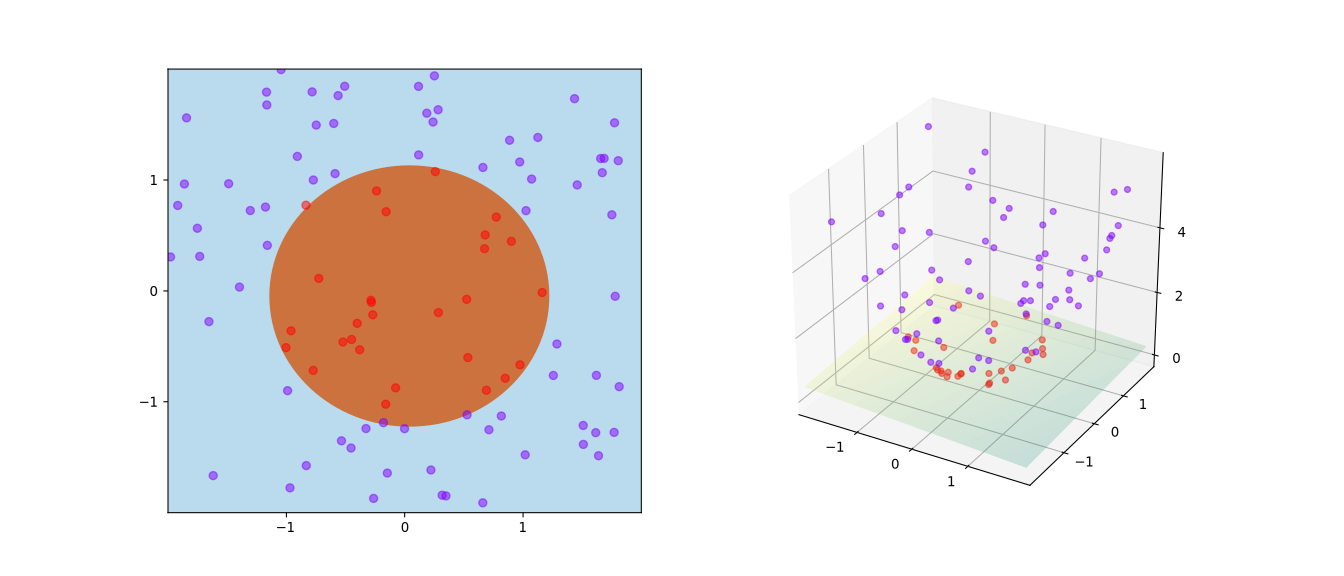
\includegraphics[width=0.6\linewidth]{Kernel_trick_idea.png}
	\caption{kernel trick idea: SVM with kernel given by $\phi(\vbx(x_1, x_2)) = (x_1, x_2, x_1^2 + x_2^2)$ and thus $\kernel(\vbx,\vbx')=\vbx\cdot \vbx' + \norm{\vbx}^2 \norm{\vbx'}^2$. The training points are mapped from a 2-dimensional to a 3-dimensional space where a separating hyperplane can be easily found. (from Wikipedia: Kernel method)}
	% that only depends on inner product
	\label{fig:kernel}
\end{figure}
% \begin{figure}[!ht]
% 	\centering
% 	\begin{subfigure}{0.3\textwidth}
% 	\centering
% 		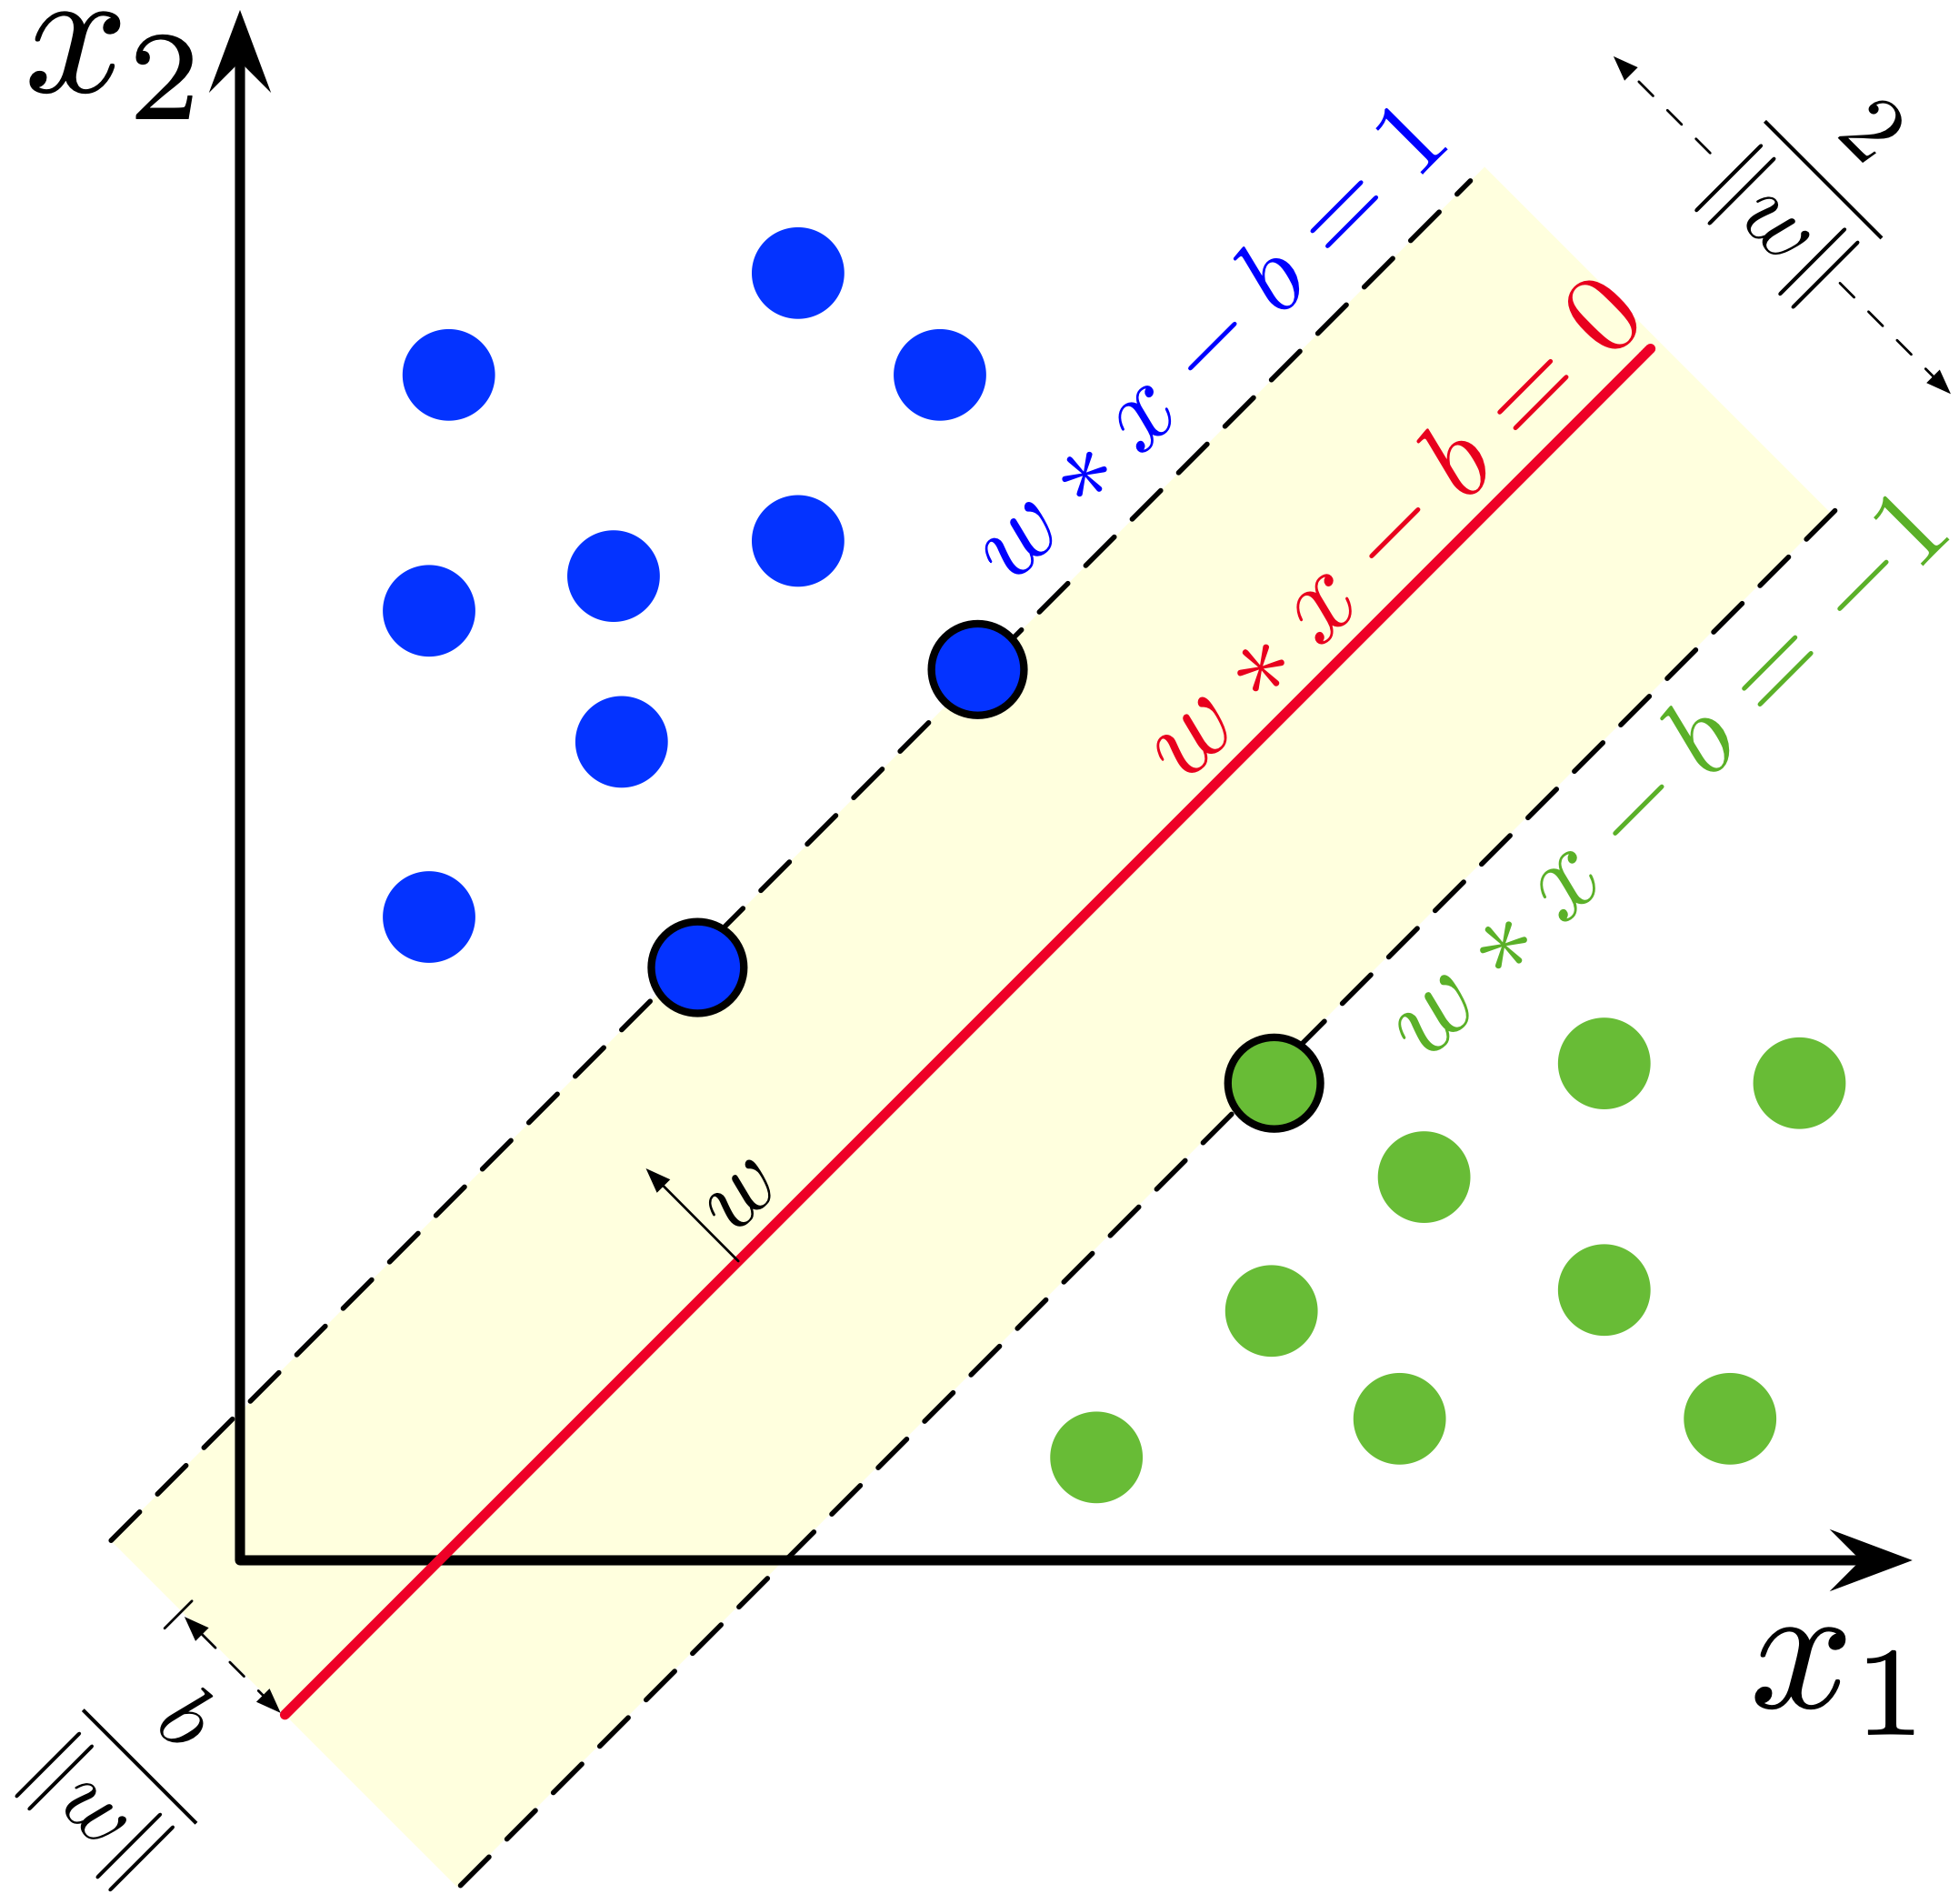
\includegraphics[width=.9\linewidth]{SVM_margin.png}
% 		\caption{linearly separable SVM}
% 	\end{subfigure}
% 	\begin{subfigure}{0.68\textwidth}
% 	\centering
% 		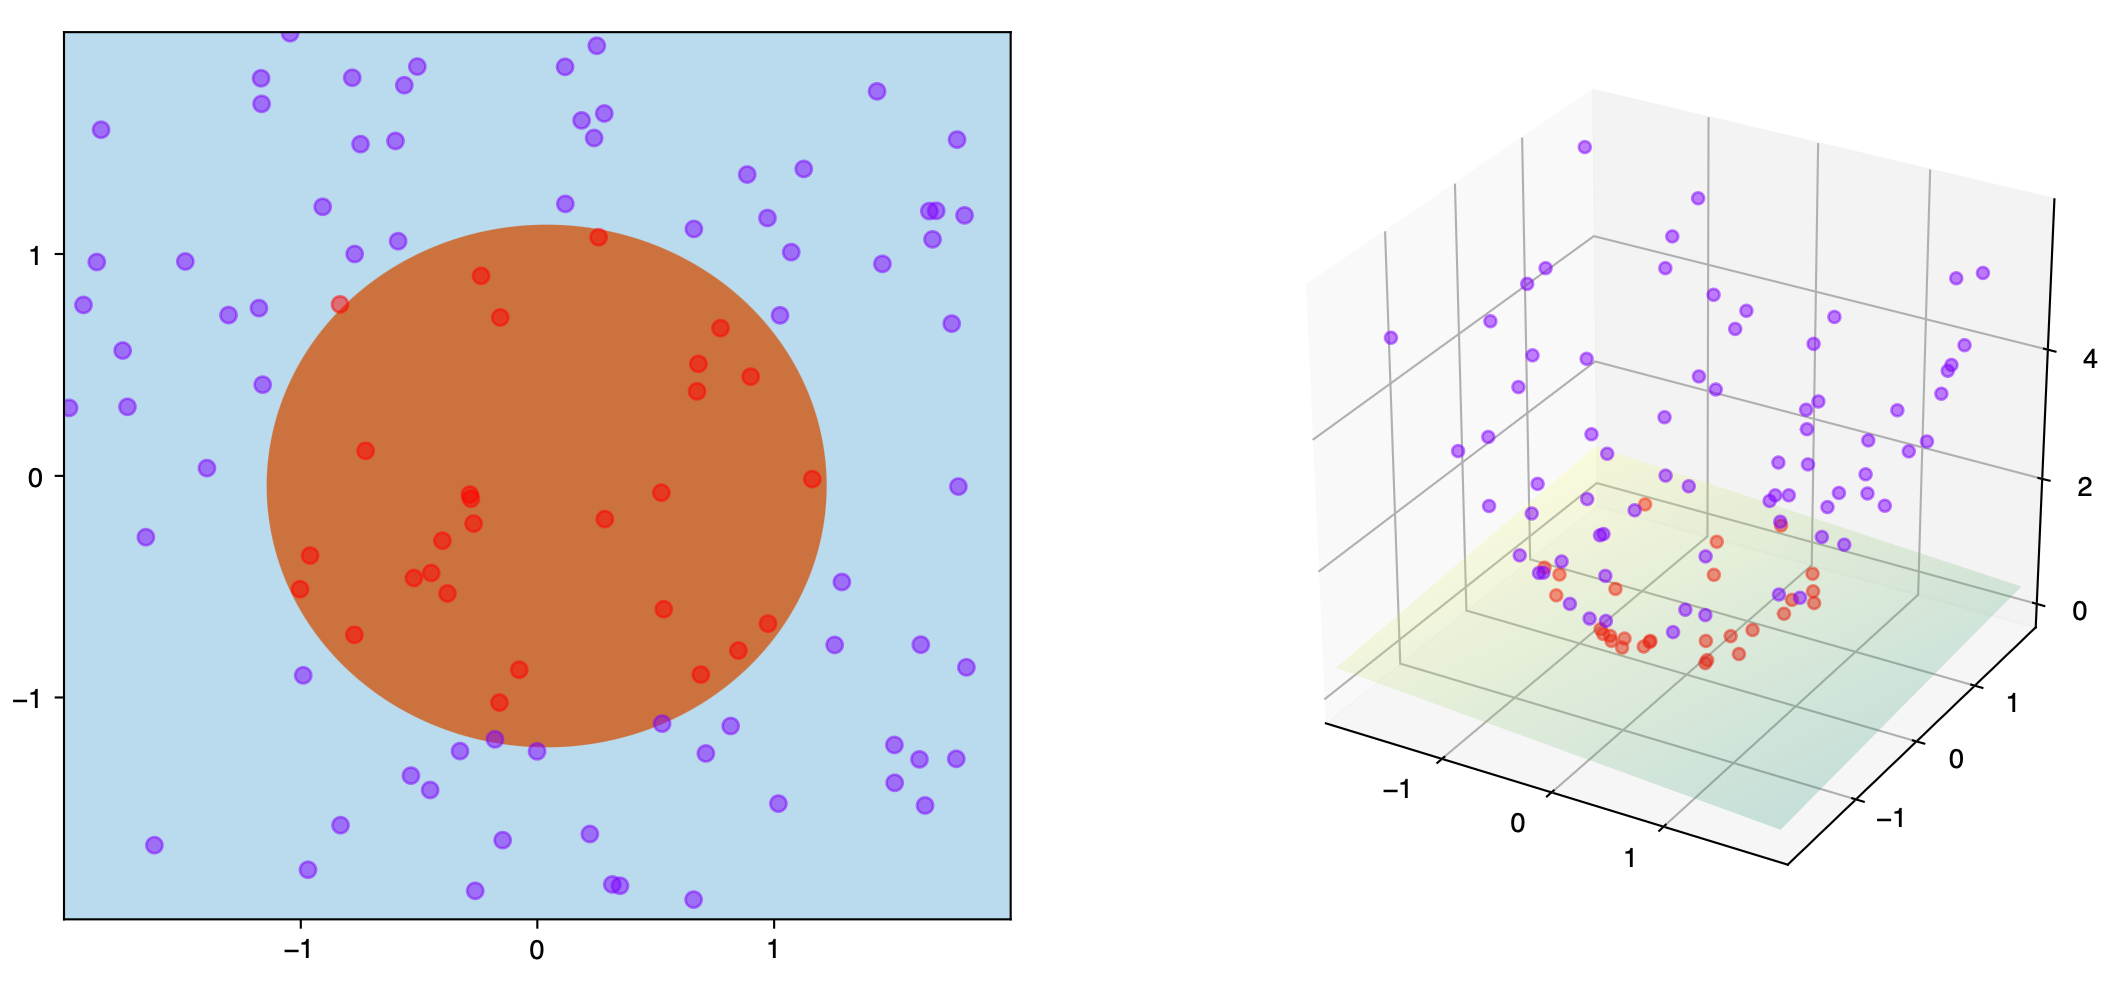
\includegraphics[width=.9\linewidth]{kernel_trick_idea.png}
% 		\caption{kernel trick idea: SVM with kernel given by $\phi(\vbx:=(a, b)) = (a, b, a^2 + b^2)$ and thus $\kernel(\vbx,\vb{y})=\vbx\cdot \vb{y}+\norm{x}^2 \norm{y}^2$ that only depends on inner product. The training points are mapped to a 3-dimensional space where a separating hyperplane can be easily found. (from Wikipedia: Kernel method)}	
% 	\end{subfigure}
% \end{figure}
\begin{example}
Some common (popular) kernels with input space $\realnumber^d$ (dot product):
\begin{itemize}
	\item \emph{polynomial kernel}:
	$\kernel(\vbx,\vbx')=(c+\vbx\cdot \vbx')^\nu$.
	Take $d=2,\nu=2$ as an example, the corresponding feature map is $\Phi(\vbx)=(x_1^2,x_2^2,\sqrt{2c}x_1,\sqrt{2c}x_2,c)^\T$.

	\item \emph{Gaussian (radial basis) kernel}:
	\begin{equation}
		\kernel(\vbx,\vbx') = 
		\exp(-\frac{\norm{\vbx-\vbx'}^2}{2\sigma^2})
		% =?
		\label{eq:gaussian_kernel}
	\end{equation}
	with the feature map $\Phi(\vbx)?=(\frac{1}{\sqrt{0!}}e^{-\vbx^2}\vbx^0,\dots,\frac{1}{\sqrt{n!}}e^{-\vbx^2}\vbx^n,\dots)$ (infinite dimensions)
	% \item Radial Kernels (Ornstein Uhlenbeck):
	% \begin{equation}
	% 	\kernel(\vbx,\vbx') = 
	% 	\exp(-\frac{\norm{\vbx-\vbx'}}{\gamma})
	% \end{equation}
\end{itemize}
\end{example}
\begin{remark}
Note that the Hilbert space associated with the Gaussian RBF kernel has infinite dimension, but the kernel may be readily computed for any pair of data points.
Since both polynomial kernel and Gaussian kernel depends only on the inner product $\vbx\cdot\vbx'$, 
no explicit calculation for the feature maps is required. 
% only depend on the inner product to avoid the expensive (exponential) calculation. [ref]
% we don't need the explicit mapping $\Phi$ as the kernel alone defines the solution 
\end{remark}
Although the development of kernel methods was driven by the empirical success of supervised learning of vector-valued data or image data, 
in many domains, such as chemo- and bioinformatics, (social) network analysis, data are not naturally interpreted as vectors.
Instead, graphs are the better representations.
In the remainder of this paper, we are going to shift our attention to graphs (inputs) instead of vectors in $ \realnumber^d$.

\section{Graph Kernels and Quantum Random Walks}
For graph-structured data, graph kernels are designed measure the similarity between graphs.
% a survey on graph kernels \cite{kriegeSurveyGraphKernels2020}.
Now, we have two basic questions:
\textbf{How similar are two vertices of a graph?}
\textbf{How similar are two graphs?}
We commence by reviewing the classical graphs kernels and then quantum random walks.

\subsection{Diffusion kernel of a pair of vertices}
Kondor and Lafferty proposed the diffusion kernel on a graph \cite{kondorDiffusionKernelsGraphs2002} that answered the question how to measure the similarity between two vertices on a graph.
It was then generalized to regularization case \cite{kondorGraphletSpectrum2009}. 
% We propose a family of regularization operators (equivalently, kernels) on graphs that include Diffusion Kernels as a special case, and show that this family encompasses all possible regularization operators invariant under permutations of the vertices in a particular sense.
% \cite{smolaKernelsRegularizationGraphs2003}

% with Euclidean space $\Omega = \realnumber^m$

\begin{definition}[Adjacency matrix]\label{def:adjacency_matrix}
	Given a (undirected, unweighted) graph $\graph=(V,E)$, its \emph{adjacency matrix} $\hat{A}$ is defined as
	\begin{equation}
		\hat{A}_{v,v'} : = 
		\begin{cases}
			1, & (v,v') \in E \\
			0, & \text{otherwise}
		\end{cases}
	\end{equation}
	where the matrix entry is 1 if the two vertices $v,v'$ (labels of the column and the row) are connected by an edge, otherwise the entry is 0.
\end{definition}
\begin{definition}[Graph Laplacian]\label{def:graph_laplacian}
	With the adjacency matrix $\hat{A}$, the graph Laplacian is obtained by
	\begin{equation}
		\llaplacian:=\hat{A}-\hat{D}	
		% \Longleftrightarrow
		% \hhat_0=\frac{\phat^2}{2m}
		% % \sim \nabla^2
		% =-\frac{\hbar^2\nabla^2}{2m}
		% % \Longleftrightarrow \dlagrangian ?
	\end{equation}
	where $\hat{D}_{v,v}:=\textup{deg}(v)=\sum_{v}[\hat{A}]_{v,v'}$ is the diagonal degree matrix.
\end{definition}
\begin{remark}
The adjacency matrix and graph Laplacian of a weighted graph can be defined in the similar manner.
% \begin{remark}
	Graph Laplacian $\llaplacian$ is the 
	discrete version of (continuous) Laplacian operator $\laplacian$
	\cite{chungSpectralGraphTheory1997}.
% \end{remark}
% \begin{observation}
	The matrix exponential of any? $\hhat$, i.e. $e^{\beta \hamiltonian}$, is a valid kernel (\psd). [to verify for $e^{-\ii t\hamiltonian}$]
% \end{observation}
\end{remark}
\begin{definition}[Diffusion kernel]\label{def:diffusion_kernel}
	The \emph{diffusion kernel} of a graph is defined as the exponential of the Laplacian
	% \cite{kondorDiffusionKernelsGraphs2002}
	% is $\kernel(v,v'):V(G)\to \realnumber$, i.e.,
	\begin{equation}
		\kernel(v,v') := 
		\qty[\sum_{k}\frac{\beta^k}{k!}\llaplacian^k]_{v,v'}  =
		\qty[e^{\beta \llaplacian}]_{v,v'} 
	\end{equation}
	where the input space $\inputspace$ is the set of vertices $V$ of graph $G$.
\end{definition}

\subsubsection{Diffusion (heat) equation, and random walks}
The continuous-time random walk on a graph is defined as the solution of the differential equation
\begin{equation}
	\dv{t} p_j(t)
	=
	\sum_{k\in V} \llaplacian_{jk} \ p_k(t),
	\label{eq:continuous_time_random_walk}
\end{equation}
where $p_j(t)$ denotes the probability associated with vertex $j$ at time $t$
and $\llaplacian$ is the \nameref{def:graph_laplacian}.
% Since the columns of $\llaplacian$ sum to 0,
% % \begin{equation}
% % 	\dv{t} \sum_{j\in V} p_j (t) = 
% % 	\sum_{j,k\in V} \llaplacian_{jk}  p_k(t) = 0
% % \end{equation}
% % which shows that 
% an initially normalized distribution remains normalized:
% the evolution of the continuous-time random walk for any time $t$ is a \emph{stochastic process}.
The simple \emph{random walk} (discrete-space, discrete-time)
% discretize the time derivative in \cref{eq:continuous_time_random_walk}
\begin{equation}
	p_j(t+1) = \frac{p_{j+1}(t) + p_{j-1}(t)}{2} 
	\label{eq:simple_random_walk}
\end{equation}
is the finite difference form of \emph{heat equation} 
\begin{equation}
	\pdv{p(t,x)}{t} = \pdv{ ^2 p(t,x)}{x^2}
	% u_t = \alpha \laplacian u \equiv \alpha \Delta u
	\label{eq:heat_equation}
\end{equation}
which is continuous-space, continous-time case.
The solution to \cref{eq:heat_equation} is called \emph{heat kernel} $\kernel(t;x,x')=\frac{1}{4\pi t} e^{-\abs{x-x'}^2/4t}$ (Gaussian).

\subsection{Continuous-time quantum random walk}\label{sec:ct_quantum_walk}
% These properties result in an exponential increase of the dimensionality of the state-space, which is the basis of the quantum speedup.
The continuous-time quantum random walk \cite{childsExampleDifferenceQuantum2002} is the quantum analogue of classical diffusion (continuous-time random walk).
By a direct observation, \cref{eq:continuous_time_random_walk} is very similar to the time-dependent (evolution) schrodinger equation governed by a Hamiltonian operator $\hamiltonian$
\begin{equation}
	\ii\hbar \dv{t} \ket{\psi} = \hamiltonian \ket{\psi}
	\label{eq:evolution}
\end{equation}
except that the factor of $\ii\hbar$.
\begin{definition}[Quantum propagator]\label{def:quantum_propagator}
	\emph{Quantum propagator} is a function that specifies the probability amplitude for a quantum particle to travel from one place to another in a given period of time.
	This propagator may also be written as the \emph{transition amplitude}.
	\begin{equation}
		\kernel (x,t;x',t')
		=
		\mel{x}{e^{-\ii (t'-t) \hamiltonian}}{x'}
		=
		\mel{x}{\U}{x'}
	\end{equation}
\end{definition}
Interestingly, this quantity is also called \emph{quantum kernel} (much earlier than the concept of kernel tricks in machine learning).
The propagator of a one-dimensional free particle can be evaluated 
\begin{equation}
	\kernel_{free}(x_I,0;x_F,t)  =
	\mel{x_F}{e^{-\ii t \phat^2/(2m\hbar) }}{x_I}
    =
	\sqrt{\frac{m}{2\pi \ii \hbar t}}
    \exp(\frac{\ii}{\hbar}\frac{m (x_F-x_I)^2}{2t}).
    \label{eq:free_propagator}
\end{equation}
by \emph{path integral (Lagrangian) formalism} (see \cref{sec:lagrangian}).
\cref{eq:free_propagator} is a Gaussian form again.

\subsection{Graph kernels of a pair of graphs}
The graph kernel of a pair of graphs was firstly proposed by Haussler \cite{hausslerConvolutionKernelsDiscrete1999}, called R-convolution kernel.
Graphs kernels are designed to compare the similarity of each of the decompositions of a pair of graphs.
Different kernels are defined, depending on how the graphs are decomposed.
Most R-convolution kernels count the number of isomorphic substructures in the two graphs.
random walk kernel (shortest paths)
\cite{vishwanathanGraphKernels2010}. 
% quantum graph kernel \cite{baiQuantumJensenShannon2015}
survey \cite{kriegeSurveyGraphKernels2020}
% \cite{chungSpectralGraphTheory1997}
\begin{definition}[Products of graphs]\label{def:product_graphs}
	The \emph{direct product of graphs}, 
	$G_{\times}(V_{\times},E_{\times}) : =G(V,E)\times G'(V',E') $
	\begin{equation}
		V_{\times}:= \qty{(v,v')\in V\times V'}
		,\quad
	% \end{equation}
	% \begin{equation}
		E_{\times}:= \qty{\qty((v_i,v_i'),(v_j,v_j'))\subseteq V_{\times}\times V_{\times}: (v_i,v_j)\in E \wedge (v_i',v_j')\in E'}
	\end{equation}
	where $V\times V'$ is the Cartesian product of two sets.
	% \begin{equation}
	% 	G_{\times} 
	% 	% : =	G(V,E)\times G'(V',E') 
	% 	: = \qty{(v,v')\in V\times V',((v,v'),(w,w')): (v,w)\in E, (v',w')\in E'}
	% \end{equation}

	% \begin{itemize}
	% 	\item 
	% 	\emph{tensor (Kronecker) product of graphs}; $G\otimes G' := \qty{ \vee }$
	% 	% \begin{equation}
	% 	% 	G\otimes G' := \qty{ \vee }
	% 	% \end{equation}

	% 	\item 
	% 	\emph{Cartesian product of graphs}; $G\times G' = \qty{}$
	% 	% \begin{equation}
	% 	% 	G\times G' = \qty{}
	% 	% \end{equation}

	% 	\item 
	% 	% \emph{Kronecker sum};
	% 	\emph{factor graph};
	% 	% \emph{Hadamard product} element-wise multiplication;
	% \end{itemize}
\end{definition}
\begin{remark}
	The adjacency matrix of the product graph $\hat{A}_{\times}=\hat{A}\otimes \hat{A}'$ and $\exp(\hat{A}_{\times})=\exp(\hat{A})\otimes \exp(\hat{A}')$.	
	Performing a random walk on the direct product graph is equivalent to performing a simultaneous random walk on $\graph$ and $\graph'$.
	However, in general, the Laplacian of the direct product graph 
	$\llaplacian_{\times}\neq \llaplacian\otimes \llaplacian'$.
\end{remark}
\begin{definition}[Graph kernel]\label{def:graph_kernel}
	Given a pair of graphs $(G,G')$,
	% \emph{random walk kernel} ?
	a \emph{graph kernel} is a function (mapping)
	$\kernel(G,G'): \qty{ \graph } \times \qty{ \graph } \to \realnumber$
	\begin{equation}
		\kernel(G,G') =
		\frac{1}{\abs{G}\abs{G'}}
		\sum_k \frac{\lambda^k}{k!} \vbe^\T A_{\times} \vbe
		=\frac{1}{\abs{G}\abs{G'}}
		\vbe^\T \exp(\beta \hat{A}_{\times}) \vbe
	\end{equation}
	where $\vb{e}$ is ...
\end{definition}
% The idea of the shortest path kernel is to compare the attributes and lengths of the shortest paths between all pairs of vertices in two graphs.
Graph kernels based on random walks count the number of (label sequences along) walks that two graphs have in common.
\begin{definition}[Random walk kernel]
	\begin{equation}
		\kernel_{\times}(G,G) = ...
	\end{equation}
\end{definition}
% \begin{remark}
\begin{definition}[Factor graph]
	\emph{factor graph} ...
\end{definition}
For diffusion processes on factor graphs, the kernel is given by the product of kernels on the constituents, that is 
\begin{equation}
	\kernel((i, i'), (j, j')) = \kernel(i, j) \kernel' (i' , j' ).
\end{equation}
% \end{remark}
\begin{remark}
	A natural question to ask is the following: since diffusion can be viewed as a \textbf{continuous time} limit of random walks, can the ideas behind the random walk kernel be extended to diffusion? Unfortunately, the Laplacian of the product graph does not decompose into the Kronecker product of the Laplacian matrices of the constituent graphs; this rules out a straightforward extension.
	Is it feasible to extend by discrete-time quantum random walk (need coin space) \cite{ambainisCoinsMakeQuantum2005} or
	Szegedy's walk formalism
	\cite{szegedySpectraQuantizedWalks2004}.
\end{remark}

\subsection{Discrete-time quantum random walk}
Discrete-time (DT) quantum random walk is the quantum analogy of classical DT random walk c.f. \cref{eq:simple_random_walk}.
The significant difference between CT and DT quantum random walk is that DT quantum random walk requires a coin space (flip a quantum coin at each move) to ensure the unitarity of the quantum walk \cite{ambainisOnedimensionalQuantumWalks2001}.
Consequently, they have different behaviors.
[TODO]

\subsection{Relations, difference, and examples}
\subsubsection{Chain}
Consider a 1-dimensional lattice (chain/line) of $N$ vertices,
the classical diffusion kernel between two positions $z_I,z_F\in [N]$
\begin{equation}
	\kernel_{\classical}(z_F,z_I) = \frac{1}{N}  
	\sum_{\nu=1}^{N} e^{-2\beta(1-\cos\frac{2\pi \nu}{N})} 
	\cos\qty(\frac{2\pi\nu(z_I-z_F)}{N}).
\end{equation}
% where $\omega_{\nu}=2(1-\cos\frac{2\pi \nu}{n})$.
\nameref{def:quantum_propagator} (CT quantum random walk)
\begin{align}
	\kernel_{\quantum}(z_F,z_I) = 
	\mel{z_F}{e^{-\ii t\hhat_0 }}{z_I}
	&=\sum_{\nu=1}^{N} 
	e^{-\ii 2t \cos\qty(\frac{2\pi}{N}\nu)} 
	\exp(\ii \frac{2\pi \nu(z_I-z_F)}{N})
	\\
	&
	% \approx \frac{1}{2\pi} \int_{\pi}^{\pi} e^{\ii p d -2\ii t cos(p)} \dd{p} 
	\approx e^{2\ii t} (-\ii)^{d} J_{d} (2t)
	\tag{large N approx}
	\label{eq:ctqrw_kernel}
\end{align}
where $J(\cdot)$ is the Bessel function and $d$ is the distance between the initial and final positions $z_I,z_F$.
\begin{figure}[!ht]
	\centering
	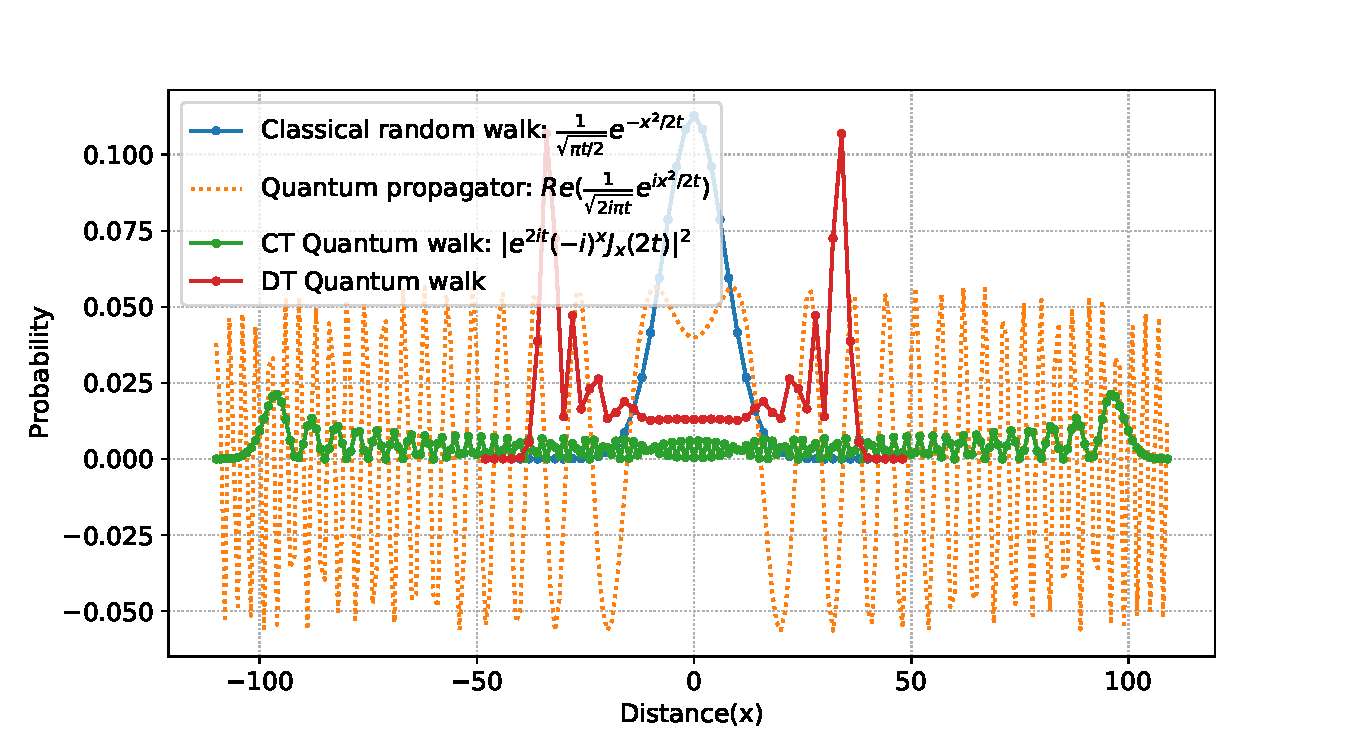
\includegraphics[width=.7\linewidth]{walk_propagator_1d.pdf}
	\caption{The probability distributions of different walks in 1d space after 50 steps.}
	\label{fig:random_walks}
\end{figure}
% The discrete-time quantum walk ...
\begin{remark}
    The random walk on this graph starting from the origin (in either continuous or discrete time)
    typically moves a distance proportional to $\sqrt{t}$ in time $t$.
	In contrast, quantum random walks spread linearly in time $t$.
	see \cref{fig:random_walks}
\end{remark}

\subsubsection{Complete graph}
the classical diffusion kernel:
$\hamiltonian_{ij}=1-\delta(i,j)N$
\begin{equation}
	\kernel_{\classical} (i,j) = 
	\frac{1-\hamiltonian_{ij} e^{-N\beta }}{N}
\end{equation}
% with increasing $\beta$, the kernel relaxes exponentially to $\kernel(i,j)=1/n$.
CT quantum random walk
\begin{equation}
	\kernel_{\quantum} (i,j) = 
\end{equation}
DT ...

\subsubsection{Hyercube}
The classical diffusion kernel on a $n$-dimensional hypercube 
\begin{equation}
	\kernel_{\classical}(\vbx,\vbx')  
	\propto
	\qty(
		\frac{1-e^{-2\beta}}{1+e^{-2\beta}}
	)^{d(\vbx,\vbx')}
	= \qty(\tanh \beta)^{d(\vbx,\vbx')}
\end{equation}
which only depends on the Hamming distance $d(\vbx,\vbx')$ between two binary strings $\vbx$ and $\vbx'$.
Quantumly, the unitary evolution operator of quantum (continuous-time) diffusion 
\begin{equation}
	e^{-\ii t \hat{A}} = 
	\prod_{j=1}^n e^{-\ii t \px^{(j)} }
	= \bigotimes_{j=1}^n
	\begin{pmatrix}
		\cos t & -\ii \sin t \\ 
		-\ii \sin t & \cos t
	\end{pmatrix}.
\end{equation}
Discrete-time ...
\cite{mooreQuantumWalksHypercube2001}
% Note 
\begin{remark}
	% In contrast, 
	Consider the continuous or discrete time random walk starting from the vertex $\vbx$. 
	The probability of reaching the opposite vertex $\bar{\vbx}$ is exponentially small at any time, since the walk rapidly reaches the uniform distribution (no stationary distribution?) over all $2^n$ vertices of the hypercube. 
	So this simple example shows that random and quantum walks can exhibit radically different behaviors.
\end{remark}

\subsubsection{Tree}
Kondor and Lafferty \cite{kondorDiffusionKernelsGraphs2002} discuss the diffusion kernel of the (infinite) 3-regular tree and binary rooted tree
\begin{equation}
	\kernel_{\classical} (i,j) = 
	\frac{1}{2} \kernel_{R}^{(3)}(d(i,j)) + \frac{1}{2} \kernel_R^{(3)} \qty(d(i,r)+d(r,j)+1)
	\tag{??}
\end{equation}
where $r$ designates the root and $d$ measures distances on the binary tree.
\begin{figure}[!ht]
	\centering
	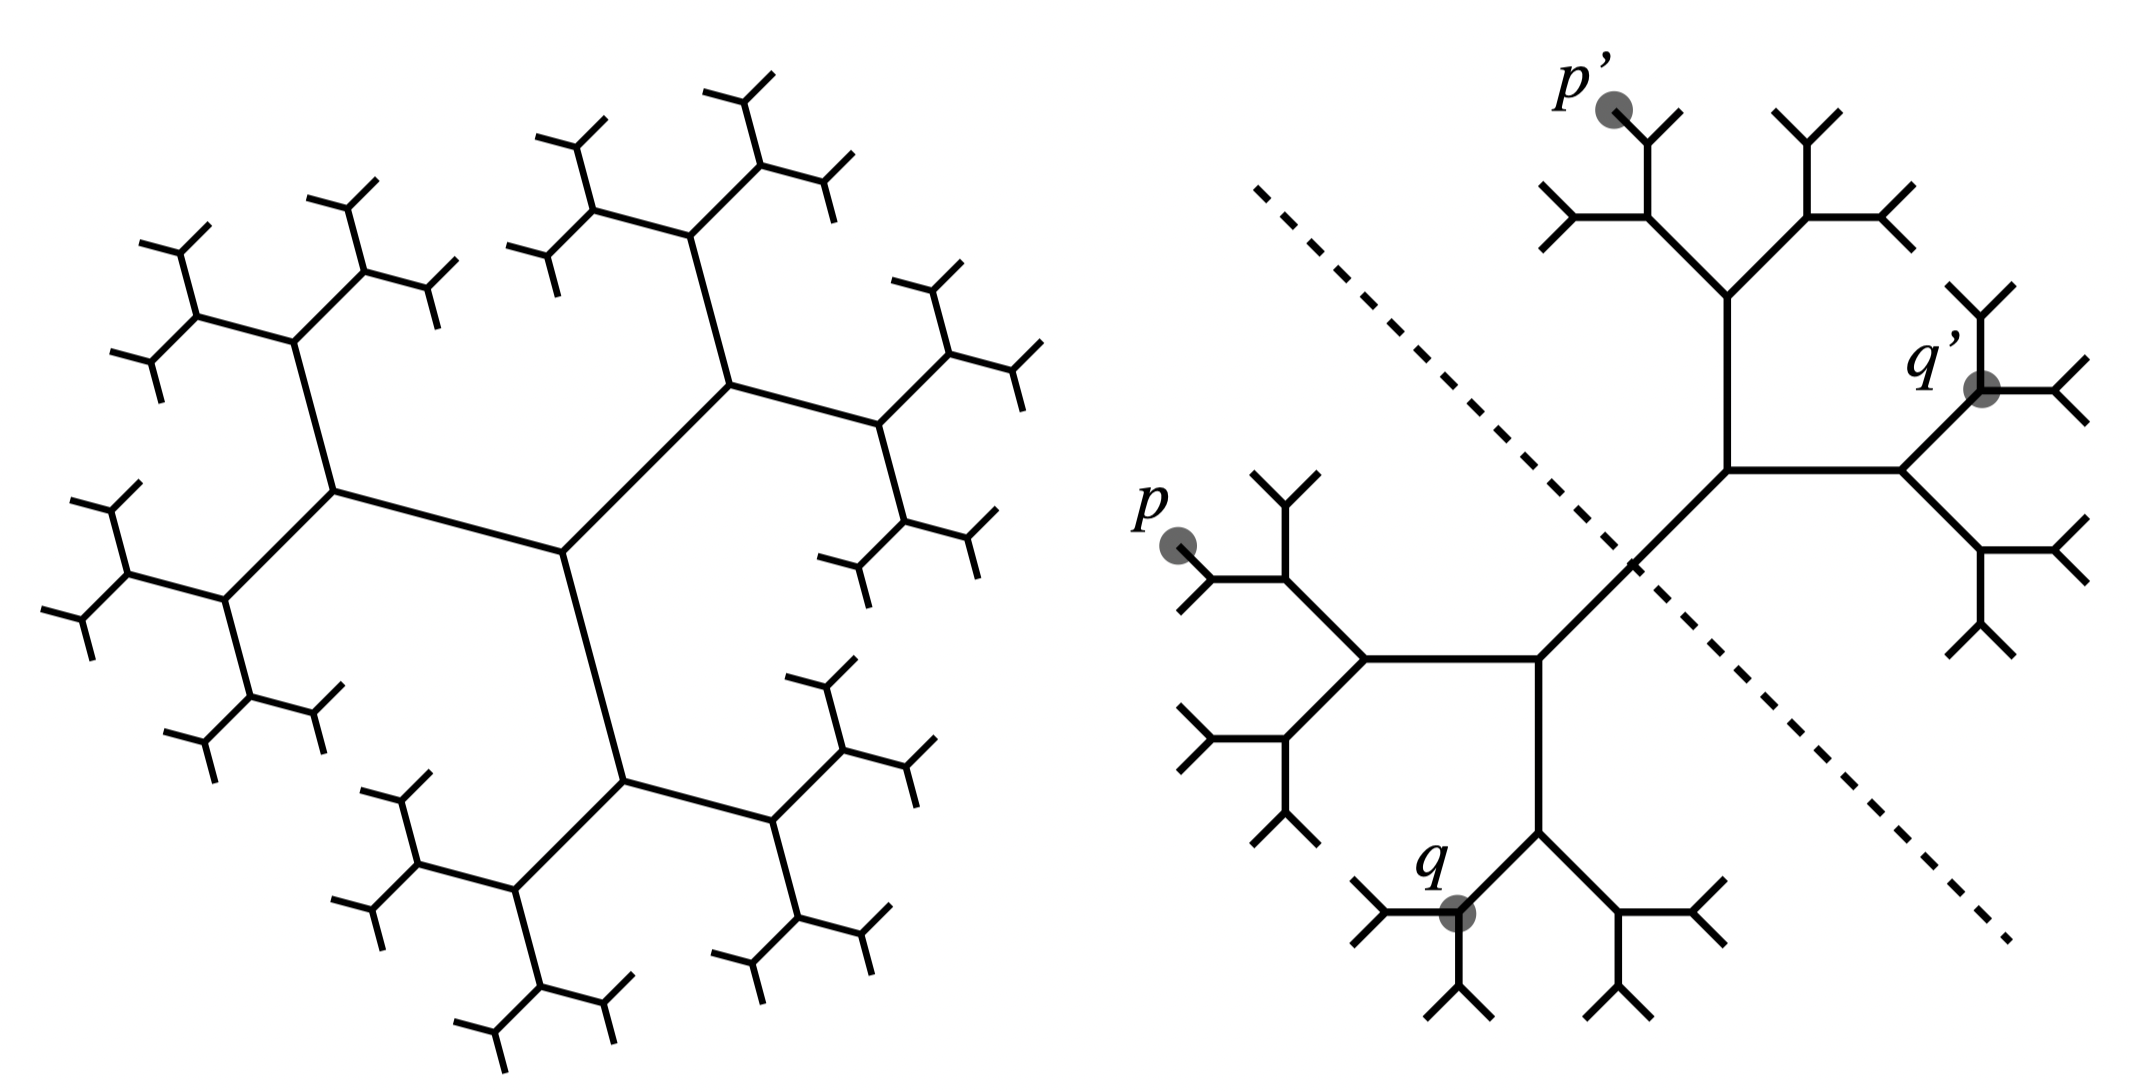
\includegraphics[width=.6\linewidth]{regular_tree.png}
	\caption{The three-regular tree (left), which extends to infinity in all directions. A little bending of the branches shows that it is isomorphic to two rooted binary trees joined at the root (right). \cite{kondorDiffusionKernelsGraphs2002}}
\end{figure}
On the other hand, Childs et. al \cite{childsExponentialAlgorithmicSpeedup2003} investigate the CT quantum random walk on another kind of tree and show an exponential speedup over classical computation.
% We have seen that the behavior of a quantum walk can be dramatically different from that of its classical counterpart. Next we will see an even stronger example of the power of quantum walk: a black-box problem that can be solved exponentially faster by a quantum walk than by any classical algorithm.
An prominent example
\begin{problem}[Glued tree]
	Consider a graph obtained by starting from two balanced binary trees of height $n$, and joining them by a random cycle of length $2\cdot 2^n$ that alternates between the leaves of the two trees. (e.g. \cref{fig:glued_tree} when $n = 4$)
	\begin{itemize}
		\item \textbf{Input:} a such glued tree in its \nameref{def:adjacency_matrix} $\hat{A}$ representation, oracle? to entries of $\hat{A}$
		% dequantization?
		\item \textbf{Output (goal):} find the exit (start from entrance)
	\end{itemize}
\end{problem}
\begin{figure}[!ht]
	\centering
	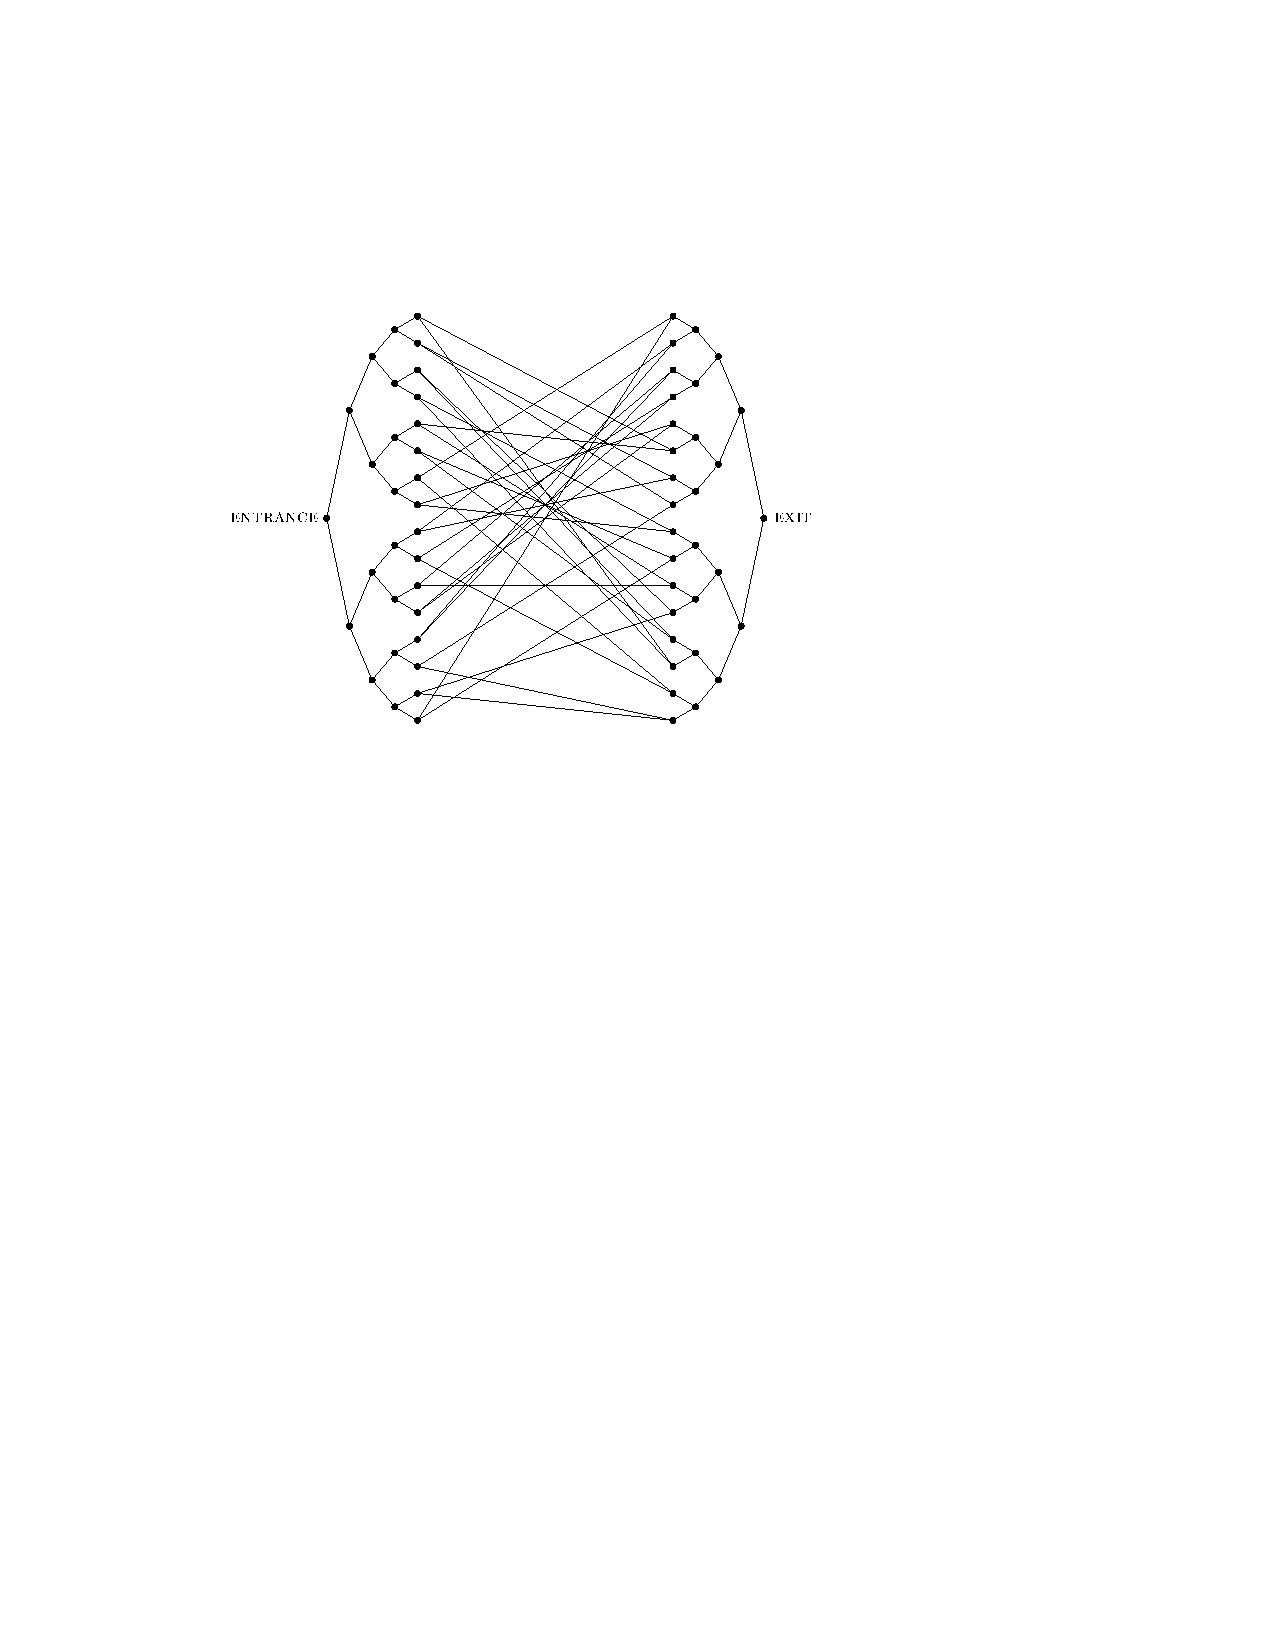
\includegraphics[width=.5\linewidth]{glued_tree.pdf}
	\caption{A typical graph exhibits exponential (query) speedup over classical model in graph matrix representation. \cite{childsExponentialAlgorithmicSpeedup2003}}
	\label{fig:glued_tree}
\end{figure}
% \begin{theorem}[\cite{childsExponentialAlgorithmicSpeedup2003}]
% 	There exists exponential (classiacl-quantum) separation with respect to query complexity under the adjacency matrix (graph) model. (glued tree)
% \end{theorem}

\subsubsection{Cayley graphs (TODO)}
\begin{definition}[Cayley graph]\label{def:cayley_graph}
	Cayley graph is a graph that encodes the abstract structure of a group. 
\end{definition}

\section{Quantum Advantages and Speedups}\label{sec:speedup}
% provide both theoretical insight and numerical demonstrations for its success, and show its feasibility for near-term experimental implementation.
% A quantum version of this approach has already been proposed in \cite{rebentrostQuantumSupportVector2014},
% where an exponential improvement can be achieved if data is provided in a coherent superposition. 

% \subsection{Quantum Machine Learning: SVM and QKE}
\subsection{Related works}\label{sec:qke}
There have been several attempts to introduce kernel method to quantum machine learning.
% theoretically sound analogs of convolutional neural networks to quantum circuits, but they have generally been somewhat heuristic.
% is highly desirable because it not only helps to gain important physical insights about the system but also leads to more efficient

\subsubsection{Quantum SVM and kernel tricks}
Quantum version of SVM was proposed \cite{rebentrostQuantumSupportVector2014} to exploit the power of quantum computer, where an exponential improvement can be achieved if data is provided in a coherent superposition. 
% \cite{havlicekSupervisedLearningQuantum2019}
It is shown that a quantum support vector machine can be implemented with $O(\log md)$ run time in both training and classification stages. 
The performance in $d$ arises due to a fast quantum evaluation of inner products.
However, when data is provided in the conventional way, i.e. from a classical computer, then the methods cannot be applied \cite{tangQuantuminspiredClassicalAlgorithm2019}.
% For the performance in M, we re-express the SVM as an approximate least-squares problem [15] that allows for a quantum solution with the matrix inversion algorithm [16, 17]. 
% We employ a technique for the exponentiation of non-sparse matrices recently developed in [18]. This allows us to reveal efficiently in quantum form the largest eigenvalues and corresponding eigenvectors of the training data overlap (kernel) and covariance matrices. We thus efficiently perform a low-rank approximation of these matrices (principal component analysis, PCA).
\begin{definition}[Quantum feature map]\label{def:quantum_feature_map}
	% the quantum state space (Hilbert space) as the feature space to still obtain a quantum advantage
	% mapping the input data non-linearly to a quantum state (density matrix) 
	The \emph{quantum feature map} is the direct quantum analogy of classical \nameref{def:feature_map_classical}.
	\begin{equation}
		\Phi(\vbx): \Omega \to \dyad{\Phi(\vbx)},
		\label{eq:quantum_feature_map}
	\end{equation}
	where the quantum state is written in the density matrix representation.
	The quantum feature map $\Phi(\vbx)$ is realized by applying a unitary quantum circuit $\U_{\Phi(\vbx)}$ to a reference state $\ket{\vb{0}}$.
\end{definition}
\begin{notation}[norm]\label{def:norm}
	Schatten p-norm $\norm{x}_p:= (\sum_i \abs{x_i}^p)^{1/p}$.
	Euclidean norm $l_2$ norm;
	Spectral (operator) norm $\norm{\vbx}_{\infty}$;
	Trace norm $\norm{A}_{\Tr}\equiv\norm{A}_{1}:=\Tr(\abs{A})\equiv\Tr(\sqrt{A^\dagger A})$, $\abs{A}:=\sqrt{A^\dagger A}$, $p=1$;
	Frobenius norm $\norm{A}_{F}:=\sqrt{\Tr(A^\dagger A)}$, $p=2$;
	Hilbert-Schmidt norm $\norm{A}_{HS}:=\sqrt{\sum_{i,j} A_{ij}^2 }=?\sum_{i\in I}\norm{Ae_i}_H^2$;
	Hilbert-Schmidt inner product $\expval{A,B}_{\textup{HS}}:=\Tr(A^\dagger B)$,
	Frobenius inner product $\expval{A,B}_{\textup{F}}:=\Tr(A^\dagger B)$?
	(in finite-dimensionala Euclidean space, the HS norm is identical to the Frobenius norm)
	Although the Hilbert-Schmidt distance is arguably not too meaningful, operationally, one can use Cauchy-Schwarz to relate it to the very natural trace distance. 
	shadow norm ...
\end{notation}
\begin{definition}[Quantum kernel estimation]\label{def:quantum_kernel}
	Straightforwardly,
	% Naturally,
	the \emph{quantum kernel estimation} is the \emph{Hilbert-Schmidt} \nameref{def:inner_product} between (feature) density matrices (c.f. \cref{eq:quantum_feature_map})
	\begin{equation}
		\kernel(\vbx,\vbx') 
		= \Tr\qty(\dyad{\Phi(\vbx)}\cdot \dyad{\Phi(\vbx')})
		= \abs{\braket{\Phi(\vbx)}{\Phi(\vbx')}}^2 = 
		\abs{\matrixel{\vb{0}}{\U^\dagger_{\Phi(\vbx)} \U_{\Phi(\vbx')}}{\vb{0}}}^2
	\end{equation}
	This is exactly a \nameref{def:quantum_propagator}.
\end{definition}
Naturally, the \emph{quantum kernel estimation}
\cite{schuldQuantumMachineLearning2019}
\cite{havlicekSupervisedLearningQuantum2019} 
has been studied to enhance the performance of quantum SVM.
There are mainly two approaches.
% Here, we propose two SVM type classifiers that process data provided purely classically and use the quantum state space as the feature space to still obtain a quantum advantage.


\subsubsection{Quantum variational classification (explicit method)}
The first one is based on variational quantum circuit: generates a separating hyperplane in the quantum feature space.
the quantum variational classifier builds on \cite{mitaraiQuantumCircuitLearning2018} \cite{farhiClassificationQuantumNeural2018} and operates through using a variational quantum circuit to classify a training set in direct analogy to conventional SVMs.
To obtain an advantage over classical approaches, it is necessary to implement a map based on circuits that are hard to simulate classically.
% The exact evaluation of the inner-product between two states generated from a similar circuit with only a single diagonal layer is $\#P$ - hard.
\begin{enumerate}
	\item a classical datum $\vbx\in\Omega$ is mapped to a quantum (feature) state by applying a unitary circuit $\U_{\Phi(\vbx)}$ to a reference (initial) state $\ket{0}^n$
	\item a \textbf{short depth quantum} circuit $W(\pmb{\theta})$.
	iteratively optimize the circuit variational parameters $\pmb{\theta}$ 
	by minizing empirical error (cost function)
	\item for binary classification, apply a \textbf{binary measurement} in $Z$-basis
	% $\qty{M_y}=2^{-1}(\identity + y \vb{f})$?
	\item to obtain the empirical distribution $p_y(\vbx)$, perform repeated measurement shots.
	then assign the label according to $p_y$?
\end{enumerate}
By the hardness assumption \cite{bremnerAveragecaseComplexityApproximate2016},
the circuit is hard to simulate classically.
The hardness of estimating the kernel with classical resources is of course only a necessary and not always sufficient condition to obtain a quantum advantage.
% not robust (heuristic)
% \begin{remark}
% 	While it may appear to be only a detail, it is important to define the feature state as the density matrix Φ(x).
% \end{remark}

\subsubsection{Quantum kernel estimation (implicit method)}
In the second method, quantum computer is used only to estimate the kernel function (matrix).
And implement a conventional (classical) SVM to generate the separating hyperplane
rather than using a variational quantum circuit.
% to generate the separating hyperplane, we use a classical SVM for classification.
% \begin{enumerate}
% 	\item the kernel $\kernel(\vbx,\vbx')$ is estimated on a quantum computer
% 	\item the quantum computer is used a second time to estimate the kernel for a new datum (test) $\vb{s}\in S$ with all the support vectors.
% \end{enumerate}

\textbf{The kernel entries are the fidelities between different feature vectors.}
The overlap can be estimated directly from the transition amplitude 
\nameref{def:quantum_kernel}.
Measuring the final state in the Z-basis R-times and record the number of $\ket{0^n}$.
The frequency of this string is the estimate of the transition probability.
% The kernel entry is obtained to an additive sampling error of $\tilde{\epsilon}$ when $\bigO(\tilde{\epsilon}^{-2})$ shots are used.


\subsubsection{Quantum graph kernels}
In \cite{baiQuantumJensenShannon2015},
% \cite{baiQuantumKernelsUnattributed2017}.
a quantum graph kernel is defined in terms of quantum Jensen Shannon as a metric of dissimilarity of graphs
density matrices associated with the evolution of continuous-time quantum random walks on graphs.
In classical information theory, the Jensen-Shannon divergence $\textup{JSD}(p,p')$ is a similarity measure between probability distributions.
% \begin{equation}
% 	\textup{JSD}(p,p')
% \end{equation}
% \begin{remark}
% 	Unfortunately, the required composite entropy for the Jensen-Shannon kernel is computed from a product graph formed by a pair of graphs,
% 	and reflects no correspondence information between pairs of vertices.
% 	As a result, the Jensen-Shannon graph kernel lacks correspondence information between the probability distributions over the graphs,
% 	and thus cannot precisely reflect the similarity between graphs[??].
% \end{remark}
Analogously, the quantum version of Jensen-Shannon divergence is defined as the distance measure between mixed quantum states (density matrices).
\begin{definition}[]
	Given a graph $\graph(V,E)$, the von Neumann entropy of $\graph$ is defined as
	\begin{equation}
		H_N (\rho_{\graph}) = -\Tr(\rho_{G}\log \rho_{\graph})
		= - \sum_{j}^{\abs{V}} \lambda_j \log \lambda_j
	\end{equation}
	where $\rho_{\graph}$ is ..random walk?? and $\lambda$ is ....
	Then,
	the \emph{quantum Jensen-Shannon divergence} of two density operators $\rho$ and $\rho'$ is defined as
	\begin{equation}
		\textup{QJSD} (\rho,\rho') = 
		H_N\qty(\frac{\rho+\rho'}{2}- \frac{1}{2}H_N(\rho)) - \frac{1}{2} H_N (\rho')
	\end{equation}
	% $D_{QJS}$ is always well defined, symmetric, negative definite and bounded, i.e., $0\le D_{QJS}\le 1$?.
\end{definition}
similarity measures? advantages? why? (isomorphism?)
\begin{definition}[divergence]\label{def:divergence}
	KL divergence (relative \nameref{def:entropy}): measure the distance (similarity) between two probability distributions:
	\begin{equation}
		\kl (P || Q) := \sum P(x) \log (P(x)/Q(x))
	\end{equation}
	symmetric version: Jensen-Shannon divergence (machine learning)
	\begin{equation}
		\jsd (P || P') := \frac{1}{2} \qty(\kl(P|| M) + \kl(P'||M))
		\equiv H_S(M)-\frac{1}{2} (H_S(P) - H_S(P') ) 
	\end{equation}
	where $M=(P+P')/2$ and Shannon \nameref{def:entropy} $H_S$.
	Analogously, quantum Jensen-Shannon divergence $D_{\qjs}$ of two density matrices can be defined...
	\begin{equation}
		D_{\qjs}(\dm||\dm'):= 
		H_V(\dm_M) - \frac{1}{2} (H_V(\dm) - H_V(\dm') ) 
	\end{equation}
	as a quantum graph kernel ($\dm$ induced by quantum random walk)
\end{definition}
\begin{remark}
	\psd
shortcomings ??
\end{remark}
\nameref{def:graph_state} is an important large class of multipartite states in quantum information,
because (connected) graph states represent a large class of genuine multipartite entangled states that have concise representations.
Typical graph states include cluster states, GHZ states, and the states involved in error correction (toric code).
	% Any connected graph state is \nameref{def:fully_entangled} state.
It worth noting that 2D cluster (rectangular lattice graph) state is the universal resource for the measurement based quantum computation (MBQC) \cite{briegelMeasurementbasedQuantumComputation2009}.
\begin{question}
	efficient? meaningful encoding of graph data/input??
	Hamiltona cycle of a graph state? vertex cover
	% Any connected graph state is fully entangled m-particle state
\end{question}
\begin{definition}[graph state]\label{def:graph_state}
	Given a simple graph (undirected, unweighted, no loop and multiple edge) $G=(V,E)$, a graph state is constructed as 
	from the initial state $\ket{+}^{\otimes n}$ corresponding to $n$ vertices.
	Then, apply controlled-Z gate to every edge, that is 
	$\ket{G}:=\prod_{(i,j)\in E}\textsf{cZ}_{(i,j)} \ket{+}^{\otimes n}$
	with $\ket{+}: = (\ket{0}+\ket{1})/\sqrt{2}$.
\end{definition}
% \begin{remark}
	An $n$-partite(qubit) graph state can also be uniquely determined by $n$ independent stabilizers, 
	$S_i:= X_i \bigotimes_{j\in n}Z_j$, 
	which commute with each other and $\forall i,S_i\ket{G}=\ket{G}$.??
	The graph state is the unique eigenstate wtih eignevalue of +1 for all the $n$ stabilizers.
	As a result, a graph state can be written as a product of stailizer projectors, $\op{G}=\prod_{i=1}^n \frac{S_i +\identity}{2}$.
	% \nameref{def:stabilizer} formalism
	% stabilizer formalism
% \end{remark}	
graph state as the quantum graph kernel ???


\begin{definition}[graph property]\label{def:graph_property}
	% The setting of graph property testing provides a natural class of partial graph properties.
	monotone ...
\end{definition}
\begin{example}[colorable]\label{exm:colorable}
	$k$-colorable is a graph property, i.e., allow for a coloring of the vertices with $k$ colors such that no two adjacent vertices have the same color.
	A graph is bipartite $\iff$ 2-colorable.
	other graph properties: isomorphism; vertex cover; Hamiltonian cycle ...
\end{example}
\begin{problem}[graph property test]\label{prm:graph_property_test}
	\textbf{promise}: the input graph either has a property, or is $\epsilon$-far from having the property, meaning that we must change at least an $\epsilon$ fraction of the edges to make the property hold.
\end{problem}
\begin{theorem}[bounds for graph property test]
\end{theorem}
\begin{question}
	\cite{montanaroSurveyQuantumProperty2018}
	Is there any graph property which admits an exponential quantum speed-up?
	\cite{ben-davidSymmetriesGraphProperties2020}
	depends on input model (query adjacency matrix/list)
	% quantum algorithms (bounds) for graph properties \cite{ben-davidSymmetriesGraphProperties2020}
\end{question}
Graphs is another kind of data which is fundamentally different from a real value vector because of vertex-edge relation and graph isomorphism.
So, graph kernel \cite{kriegeSurveyGraphKernels2020} need additional attention.
\begin{definition}[graph kernel]\label{def:graph_kernel}
	given a pair of graphs $(\graph,\graph')$,
	\emph{graph kernel} is $\kernel (\graph,\graph')  =$.
	% \begin{equation}
	% \end{equation}
	quantum graph kernel $\kernel (\graph,\graph')  = \abs{\ip{\graph}{\graph'}}^2$ ??
	\cite{baiQuantumJensenShannon2015}	
\end{definition}
classical graph data mapped to graph state, then fidelity represents a kernel function??.
\begin{theorem}
	On quantum computers, evaluating the trace distances is probably hard since even judging whether $\dm$ and $\dm'$ have large or small trace distance is known to be QSZK-complete \cite{watrousQuantumComputationalComplexity2008}, where QSZK (quantum statistical zero-knowledge) is a complexity class that includes BQP (bounded-error quantum polynomial time).
	% Variational Quantum Algorithms for Trace Distance and Fidelity Estimation
\cite{chenVariationalQuantumAlgorithms2022}
\end{theorem}
\begin{proposition}[\cite{huangPowerDataQuantum2021}]
	If a classical algorithm without training data can compute (label) $y=f(x)=\mel{x}{\U_{\textup{QNN}}^\dagger \ob U_{\textup{QNN}}}{x}$ (with amplitude encoding) efficiently (poly time in ...) for any $\U_{\textup{QNN}}$ and $\ob$, then $\nameref{def:bpp}=\nameref{def:bqp}$ (which is believed unlikely).
\end{proposition}
\begin{proposition}[\cite{huangPowerDataQuantum2021}]
	Training an arbitrarily deep quantum neural network $\U_{\qnn}$ with a trainable observable $\ob$ is equivalent to training a \nameref{def:quantum_kernel} method with kernel $k_{Q}(\vbx,\vbx')=\Tr(\dm(\vbx)\dm'(\vbx'))$
\end{proposition}

\subsubsection{Quantum diffusion map}
Inspired by random walk on graphs, \emph{diffusion map} (DM) \cite{sornsaengQuantumDiffusionMap2021} is a class of \textbf{unsupervised} machine learning that offers automatic identification of \textbf{low-dimensional data structure hidden in a high dimensional dataset}.
Though both of SVM and DM are machine learning techniques that utilize kernel tricks, DM is designed for dimension reduction, the `reverse direction' of the kernel trick in SVM.
Like other dimension reduction technique, DM entails the calculate the eigenvalue/vectors (SVD).
% Most dimensionality reduction methods require the computation of singular value decomposition (SVD) of a matrix constructed from a collection of high-dimensional data points. $\bigO(N^3)$
Thus, classical dimensionality reduction can be computationally prohibitive for a large data sample. 
However, under moderate assumptions of accessibility to certain features of full-scale quantum computers, matrix exponentiation-based quantum algorithms have been proposed to perform SVD more efficiently [ref]. 
% \begin{remark}
% 	Although the backbone of DM is a graph-based dimensionality reduction method, the procedure is different from other spectral graph methods. 
% 	Namely, rather than working with the data-induced graph Laplacian as in Laplacian eigenmaps or in spectral clustering, DM involves Markov transition matrix that defines random walks on a data-induced graph.
% \end{remark}
The quantum diffusion map (qDM) consists of 5 major steps: 
\begin{enumerate}
	\item \nameref{def:coherent_state} data encoding scheme, 
	\item 
	a natural construction of kernel matrix from coherent states, 
	\cref{eq:diffusion_map_kernel}
	\item 
	a scheme to construct the Markov transition matrix from the kernel matrix, 
	\item 
	the eigen-decomposition of the transition matrix (quantumly $\bigO(\poly\log N)$?); classically $\bigO(N^3)$
	\item 
	and extracting relevant quantum information to construct diffusion map classically. 
	and classically constructs the diffusion map via the readout (tomography) of the eigenvectors, giving a total expected runtime proportional to $N^2 \poly\log N$.
\end{enumerate}
% The expected time complexity of qDM is $N^2 \poly\log N$, compared to the worst-case runtime $\bigO(N^3 )$ of a classical DM. 
% Importantly, from accessing of qRAM to performing an eigendecomposition of the Markov transition matrix, the total time complexity is only $\bigO(\log^3 N)$.
% Given the normalized (similarity) matrix $M$, 
% compute the $k$ largest eigenvalues(vectors) of $M^t$.
Rather than using mere Euclidean distance as a similarity measure between data points, manifold learning approach assigns the connectivity among data points in their neighborhood as a proxy for proximity between points.
% \begin{remark}
% 	Two points whose squared distance exceed this bandwidth contribute exponentially little to the weighted edge, suggesting that these two points are far away from being a neighbor in its original feature space.
% \end{remark}
In DM, the similarity matrix between a pair of data vectors, or equivalently the weighted edge between a pair of graph vertices, is often taken to be a Gaussian kernel \cref{eq:gaussian_kernel}:
\begin{equation}
	W_{ij}:=\kernel (\vbx^{(i)},\vbx^{(j)}) =
	\exp(-\frac{\norm{\vbx^{(i)}-\vbx^{(j)}}_2^2}{2\sigma})
	\label{eq:diffusion_map_kernel}
\end{equation}
where the adjustable parameter $\sigma$, called the bandwidth, sets the scale of neighborhood.
Given a graph with weighted edges $W_{ij}$, DM assigns a \emph{discrete-time random walk} on a data-induced graph, 
where the Markov transition probability from vertex $i$ to $j$ is given by the normalized weighted edge,
\begin{equation}
	P_{ij} = \frac{W_{ij}}{\sum_{j}W_{ij}}
	,\quad
	\tilde{P} = D^{-1} W.
\end{equation}
% \begin{remark}
% 	The notion of proximity based on graph connectivity can be characterized by how fast random walkers on a graph starting at different data points visit each other. One expects that two points that are connected by multiple paths should be near; whereas two points that are sparsely connected should lie far from each other.
% \end{remark}

% Use the diffusion map to get the embedding $\Psi_t$.
% \begin{equation}
% 	P, L
% \end{equation}
\begin{definition}[Coherent state]\label{def:coherent_state}
	A \emph{coherent state} is ...
	\begin{equation}
		\ket{\alpha} 
		% = \sum_{n=0}^{\infty} \ket{n} \braket{n}{\alpha}
		= e^{-\frac{1}{2}\abs{\alpha}^2} \sum_{n=0}^{\infty} \frac{\alpha^n}{\sqrt{n!}} \ket{n} 
		= e^{-\frac{1}{2}\abs{\alpha}^2} e^{\alpha\acreation}\ket{0} 
	\end{equation}
	where $\ket{n}$ basis and $\acreation$ is the creation operator [ref].
	% displacement operator
	% \begin{equation}
	% 	\hat{D}(\alpha)\ket{0} : = e^{\alpha \acreation - \alpha^* \aannihilation} \ket{0} = \ket{\alpha}
	% \end{equation}
\end{definition}
Consider two $n$ tensor product of (canonical) coherent states
\begin{equation}
	\ket{\pmb{\alpha}} = \ket{\alpha_{1}} \otimes\ket{\alpha_{2}} \cdots\otimes\ket{\alpha_{n}} 
	,\quad
	\ket{\pmb{\alpha}'} = \ket{\alpha_{1}'} \otimes\ket{\alpha_{2}'} \cdots\otimes\ket{\alpha_{n}'} 
\end{equation}
with $\vbx=(\alpha_1,\alpha_2,\dots,\alpha_n)$ and $\vbx'=(\alpha_1',\alpha_2',\dots,\alpha_n')$, the kernel reads 
\cite{chatterjeeGeneralizedCoherentStates2017}
\begin{equation}
	\abs{\braket{\pmb{\alpha}}{\pmb{\alpha}'}}^2 = 
	\exp(-\norm{\vbx-\vbx'}^2) 
\end{equation}
which is the Gaussian kernel c.f. \cref{eq:gaussian_kernel} and \cref{eq:diffusion_map_kernel}.
% One of the most significant limitations of classical algorithms using non-linear kernels is that the kernel function has to be evaluated for all pairs of input feature vectors which themselves may be of substantially high dimension. [quantum parallelism (superposition) measurement]
% The key link will be the \nameref{def:rkhs} property for SVMs that naturally arise from canonical and generalized coherent states. 
% Specifically, we discuss the fast evaluation of radial kernels through a positive operator valued measure (POVM) on a quantum optical system based on canonical coherent states.
% The quantum DM proposed by \cite{sornsaengQuantumDiffusionMap2021} takes as an input $N$ classical data vectors, 
% performs (quantumly) an eigen-decomposition of the Markov transition matrix in time $\bigO(\log^3 N)$, 


\subsection{Provable quantum speedups}
The core challenge to provable quantum speedup and substantial improvement for practical problems

\subsubsection{Quantum linear algebra toolbox (subroutines)}
% \cite{sornsaengQuantumDiffusionMap2021}
Firstly, provable speedups by quantum linear algebra algorithms:
\begin{itemize}
	\item HHL (quantum) algorithm for solving linear equation systems \cite{harrowQuantumAlgorithmSolving2009}, qSVD (eigen decomposition) \cite{gilyenQuantumSingularValue2019}; 
	quantum linear algebra (qMAT) \cite{zhaoCompilingBasicLinear2019}: matrices multiplication, matrix inversion, matrix exponentiation, 

	\item quantum (evolution) simulation techniques: product formula, LCU, etc.

	\item quantum Fourier transform (QFT), quantum phase estimation.

	\item FFT by quantum algorithms: 
	It is shown that quantum circuits are a natural choice for Fourier space neural architectures affording a super-exponential speedup in computing the matrix elements of $\mathbb{S}_n$-Fourier coefficients compared to the best known classical (FFT) over the symmetric group. \cite{zhengSpeedingLearningQuantum2022}
	\cite{kondorGraphletSpectrum2009}
\end{itemize}

\subsubsection{Quantum Fourier Transform (QFT) and algebraic problems}
hidden subgroup problem solved by quantum Fourier transformation\cite{childsQuantumAlgorithmsAlgebraic2010};
rigorous and robust quantum speedup with Discret Logarithm problem \cite{liuRigorousRobustQuantum2021} \cite{glickCovariantQuantumKernels2021}
\begin{problem}[Hidden subgroup problem]\label{prm:hidden_subgroup}
	Given a group $\group$ and a black-box function $f:\group\to S$, 
	$f$ is promised to satisfy 
	\begin{equation}
		f(x) =f(y) \iff x^{-1}y \in \subgroup 
	\end{equation}
	for some unknow subgroup $\subgroup \le \group$.
	We say such a function $f$ hides a subgroup $\subgroup$.
	The goal of \emph{hidden subgroup problem} (\hsp) is to learn $\subgroup$
	(specified in terms of a generating set) using queries to $f$.
\end{problem}
\begin{problem}[Simon's problem]
	The \emph{Simon's problem}, is formulated as 
	\begin{itemize}
		\item \textbf{Input}: a (partial/promise) black-box Boolean function $f:\qty{0,1}^n \to \qty{0,1}^m$ 
		% where $m$ can possibly be larger than 
		\item \textbf{Promise}: there exist a secret $s\in \qty{0,1}^n $ such that $f(x)=f(y)$ \iff $x=y$ or $x=y+s$
		\item \textbf{Output}: the value of $s$
	\end{itemize}
\end{problem}
\begin{problem}[Supervised learning with group?]
	with group structure
	\begin{itemize}
		\item \textbf{Input}: a dataset $\qty{\vbx^{(i)},y^{(i)}}_{i=1}^m$,
		that is a (partial) black-box function $f(\vbx):\qty{0,1}^n \to \qty{0,1}$
		\item \textbf{Promise}: $f(\vbx)=f(\vb{y})$ \iff $\vbx^{-1}\vb{y}\in \subgroup$
		\item \textbf{Output}: learn $f$; learn subgroup (translation?; physics?); predict $f(\vb{z})$
	\end{itemize}
\end{problem}
\begin{remark}
	Simon's problem \cite{simonPowerQuantumComputation1997}
	% (Abelian subgroup problem) 
	is a $\hsp$ with $\group = \integer^n_2$ and $\subgroup = \qty{ 0, s }$ for some $s \in \integer_2^n$ .
	Decision version of Simon's problem is Element distinctness.
	translation group?
\end{remark}
% robust, provable speedup \cite{liuRigorousRobustQuantum2021}
\begin{problem}[Discrete Logarithm problem]\label{prm:dlog}
	The \emph{discrete logarithm problem} (\dlog) is defined as
	\begin{itemize}
		\item \textbf{Input:} a prime $p$, a primitive element (generator) $g$ of $\integer_p^*:=\qty{1,2,\dots,p-1}$, and an element $y=g^x \pmod{p} \in\integer_p^*$ with some unknow $x$. black-box function $f$?
		\item \textbf{Output (goal):} find $x=\log_g y$
	\end{itemize}
	$\dlog$ is a special case of $\hsp$ with ... subgroup 
\end{problem}
reducible to decision version $\dlog_{1/2}$, then classification version.
\begin{equation}
	\dlog \le \dlog_{\textup{decision}} \le \dlog_{\textup{promise}}
\end{equation}
$\le$ represents polynomial (time) reduction.

covariant quantum kernels for the data with group structures
\cite{glickCovariantQuantumKernels2021}.
% The feature states are intimately related to covariant measurements?
% Examples could constitute learning permutations or classifying translations or rotations. 
Exploiting group structure and learning problems for group data have already been investigated for classical kernels \cite{kondorGroupTheoreticalMethods2008}.
The fiducial state $\ket{\phi}$ is chosen as some reference state from the representing Hilbert space. 
In principle, any state that can be prepared efficiently may be chosen. 
However, the choice will greatly affect the performance of the classifier as we will discuss shortly.
\begin{definition}[Covariant]\label{def:covariant}
	\emph{covariant}
	feature map circuits that we call covariant feature maps. 
\end{definition}
\begin{problem}[labeling cosets with error]
	\emph{labeling cosets with error}
	% kernel alignment?
	\begin{itemize}
		\item 
		\textbf{Input:} given a group $\group$ and subgroup $\subgroup$,
		we can define two left-cosets $\mathbb{C}_{\pm}=c_{\pm}\subgroup$ by choosing $c_+,c_-$ randomly ...
		\item 
		\textbf{Output: ?} 
	\end{itemize}
	% this problem is related to the problem of deciding membership in a subgroup
\end{problem}

\subsubsection{Permutation, symmetry, and graph properties}
It is well-known that structure of a problem is necessary for quantum speedup \cite{aaronsonNeedStructureQuantum2014}.
only polynomial speedup for total problem \cite{bealsQuantumLowerBounds2001} \cite{aaronsonQuantumImplicationsHuang2020}.
% \cite{huangInducedSubgraphsHypercubes2019}
An illustrative example is that quadratic speedup is optimal for unstructured (Grover) search \cite{groverQuantumMechanicsHelps1997}, while exponential speedup is widely believed for integer (prime) factorization (promise/partial problem) \cite{shorPolynomialTimeAlgorithmsPrime1997}.
Moreover, fully symmetric (partial) functions do not admit exponential quantum speedup in the query model.
\cite{ben-davidSymmetriesGraphProperties2020}.
% \cite{zhengSpeedingLearningQuantum2022};
% robust, provable speedup
% \cite{liuRigorousRobustQuantum2021}
A natural class of problems with significant symmetry, though much less than full permutation symmetry, is the class of graph properties. For such problems, the input describes a graph, and the output depends only on the isomorphism class of that graph. 
% \cite{childsCanGraphProperties2020}
Graph property test ...
\begin{equation}
	\le 
\end{equation}
reduction to (modified) glued tree \cref{fig:glued_tree}

% \subsubsection{Dequantization and input assumption}
% If we assume we can efficiently perform $l^2$-norm samples of input data, a natural analogue to quantum algorithms that assume efficient state preparation of classical data.
% Since they are only polynomially slower, these algorithms suggest that the exponential speedups of their quantum counterparts are simply an artifact of state preparation assumptions.
% \cite{tangQuantuminspiredClassicalAlgorithm2019}
% \cite{tangQuantumPrincipalComponent2021}
% % \begin{remark}
% % 	However, when data is provided in the conventional way, i.e. from a classical computer, then the methods of [15] cannot be applied.
% % \end{remark}
% input model, quantum RAM;
% quantum-inspired 
% % \cite{tangQuantuminspiredClassicalAlgorithm2019}
% % \cite{tangQuantumPrincipalComponent2021}.
% \cite{rebentrostQuantumSupportVector2014} \cite{lloydQuantumPrincipalComponent2014} etc need quantum state preparation assumptions, which state that given an input vector $v$, one can quickly form a corresponding quantum state $\ket{v}$. 

\subsection{Heuristic quantum advantages for learning physics systems}
Previous works evaluate the performance on the standard graph datasets from both bioinformatics and computer vision.
Instead, we could exploit the structures inherent in physics systems and make use of quantum advantages.
% problems of practical interest,
% not guaranteed.

\subsubsection{Classical machine learning for quantum physics problem}
Aligned with the development of quantum machine learing, classical machine learning is being applied to tackle quantum many-body physics (determining phase (transition)) and particle physics.
It is shown that a standard feed-forward neural network can be trained to detect multiple types of order parameter directly from raw state configurations sampled with Monte Carlo \cite{carrasquillaMachineLearningPhases2017}.
% what if one was presented with a data set of Ising configurations from an unknown Hamiltonian, where the lattice structure (and therefore its T c) is not known?
Moreover, the application of such techniques to problems of greater interest in modern condensed matter, such as disordered or topological phases, where no conventional order parameter exists.
\cite{carleoSolvingQuantumManyBody2017}
% Ising lattice gauge theory, one of the most prototypical examples of a topological phase of matter.
\begin{remark}
	A straightforward implementation of supervised training fails to classify a test set containing samples of the two states to an accuracy over 50\% - equivalent to simply guessing. Such failures typically occur because the neural network overfits to the training set. 
	To overcome this difficulty we consider a convolutional neural network (CNN) [ref] which readily takes advantage of the two-dimensional structure of the input configurations, as well as the \textbf{translational invariance} of the model.
	% \cite{carrasquillaMachineLearningPhases2017}
\end{remark}

\subsubsection{Groups and symmetries in physics and machine learning}
\citetitle*{kondorGroupTheoreticalMethods2008}
\cite{kondorGroupTheoreticalMethods2008};
\citetitle*{bogatskiyLorentzGroupEquivariant2020}
\cite{bogatskiyLorentzGroupEquivariant2020};
\citetitle*{bogatskiySymmetryGroupEquivariant2022}
\cite{bogatskiySymmetryGroupEquivariant2022};

% \subsubsection{Group theory and machine learning}
% \cite{kondorDiffusionKernelsGraphs2002}
One of the key properties of classical CNNs is equivariance, which roughly states that if the input to the neural network is shifted, then its activations translate accordingly. 
\cite{cohenGroupEquivariantConvolutional2016}
\cite{kondorCovariantCompositionalNetworks2018}
\begin{definition}[Covariant]
\end{definition}
\begin{definition}[Invariant]
	informal
\end{definition}
\begin{definition}[Equivariant]\label{def:equivariant}
	Given a group $\group$ and the actions $\rho: \group \times X\to X$ and $\rho': \group \times Y\to Y$,
	a map $f: X\to Y$ is said to be \emph{equivariant} if
	\begin{equation}
		\forall x\in X, g\in \group,
		f(\rho(g,x)) = \rho'(g,f(x))
		% f(\rho_g(x)) = \rho_g'(f(x))
	\end{equation}
	% here the notation is $\rho_g(x) = \rho(g,x)$.
\end{definition}
From equation  we see that the familiar concept of invariance is a special kind of equivariance where $T_g'$ is the identity transformation for all $g$, $f(T_g(x))=f(x)$.
% There have been several attempts to introduce theoretically sound analogs of convolutional neural networks to quantum circuits, but they have generally been somewhat heuristic.
\begin{remark}
% Equivariance is one of the main reasons behind the unreasonable success of CNNs.
% Combining these two is the basis of so-called Permutational Quantum Computing (PQC) [30]. Therefore, a natural starting point for realizing convolutional neural networks in quantum circuits is to look for permutational equivariance.
% the quantum Fourier space activation (within PQP+) enjoys a super-exponential quantum speed-up compared with the best-known result in classical FFT over the symmetric group.
	In particular, it has been recognized that by constructing neural networks that operate on the basis of irreducible representations of the group (so-called Fourier space neural networks), and group equivariant convolution is easy to implement because it simply reduces to matrix multiplication.
	The major difficulty is that the key ingredient of the success of CNNs - translation invariance - lacks a mathematically rigorous quantum counterpart due to the discrete spectrum of spin-based quantum circuits.
	the natural form of equivariance in quantum circuits is permutation equivariance.
	\cite{zhengSpeedingLearningQuantum2022}!?
\end{remark}
invariant and equivariant graph nn
\cite{maronInvariantEquivariantGraph2019}

% equivariant CNN 
% Quantum CNN \cite{congQuantumConvolutionalNeural2019} for quantum phase recognition and quantum error correction.
% The MERA framework provides an efficient tensor network representation of many classes of interesting many-body wavefunctions, including those associated with critical systems.
% The QCNN circuit has similar structure, but runs in the reverse direction.
% In this sense, the QCNN circuit can mimic renormalizationgroup (RG) flow, a methodology which successfully classifies many families of quantum phases 29.


\section{Experiments}\label{sec:experiments}

\subsection{Datasets and benchmark}
Firstly, we will validate our method (by preliminary experiment) on artificial data (of group structures).
Then, we test the performance for prototypical machine learning tasks and physics datasets.

\subsubsection{Synthetic data}
We generate artificial data that can be fully separated by our feature map.

\subsubsection{Real-world dataset}
conventional graph datasets
\begin{itemize}
	\item UCI \cite{kondorDiffusionKernelsGraphs2002}, 
	\item protein [ref], \cite{jumperHighlyAccurateProtein2021}
	\item The MUTAG dataset consists of graphs representing chemical compounds labeled ..;
\end{itemize}
physics datasets
\begin{itemize}
	\item particle physics: JET tagging task (This is a classification task that aims to identify top quark “jets” among a background of lighter quarks. Since the classification task is independent of the inertial frame of the observer, the outputs of the classifier should be \textbf{Lorentz invariants}.) \cite{bogatskiyLorentzGroupEquivariant2020}
	% All activations in our neural network will belong to various finite-dimensional representations of the Lorentz group.
	% Our goal is to design an architecture that can learn arbitrary equivariant maps between finite-dimensional representations of the Lorentz group.
	% As demonstrated in (Cohen & Welling, 2016), the restriction to equivariant linear layers, compared to a general fully connected linear layer, leads to significantly fewer learnable parameters
	% Dot products are the invariant parts in the isotypic decompositions of tensor products of two 4-vectors, therefore a quantity of this kind can be very efficiently learned by an equivariant network if physically appropriate nonlinear activation functions are chosen.
	% When a particle decay event produces hundreds of observed particles, generating all relevant Lorentz invariants (and even more so equivariants) up to a fixed polynomial degree quickly becomes an intimidating task that begs for a procedural solution. This is exactly the goal of our architecture.

	\item quantum many-body physics: determine phase transition
	\cite{carrasquillaMachineLearningPhases2017},
	topological order
	\cite{congQuantumConvolutionalNeural2019}
% \cite{dohertyIdentifyingPhasesQuantum2009} 
\end{itemize}

\section{Discussion and Conclusion}\label{sec:discussion}
% to do 
\begin{itemize}
	\item formalize quantum graph kernels (algorithm) with quantum random walk, provable speedup
	\item quantum graph kernel for the data with group structures
	\item quantum machine learning for (practical dataset) physics problem (symmetries)
	\item whether low-depth circuit for NISQ. analog computing?
\end{itemize}
\cite{ben-davidSymmetriesGraphProperties2020}


\addcontentsline{toc}{section}{References}
\printbibliography
\appendix

\section{Machine Learning and Group Theory [TODO]}
% \subsection{Kernel trick in machine learning}
\begin{itemize}
	\item supervised learning (classification, regression):
	SVM, neural network. (methods: gradient descent, backpropagation)

	\item unsupervised learning (clustering, dimension reduction): k-means, PCA

	\item reinforced learning not covered in this paper.
\end{itemize}

\subsection{Machine learning}
% training set, test set.
% find $f\in C$ classifier, hypothesis (concept) class. (unknow probability distribution)
% The algorithm consists of two main parts: a training stage and a classification stage. 
% For the training stage, a set of labeled data points are provided, on which the algorithm is performed. 
% For the classification stage, we take a different set of data points and run the optimized classifying circuit on them without any label input.

\subsubsection{Details of SVM and kernel tricks [TODO]}
% maximize the \emph{margin} [ref]
% \begin{equation}
% 	f^* = \arg \max_f  L(y,\tilde{y}) + \norm{}
% \end{equation}
% $\tilde{y}:=f(x)$.
% where the loss function $L$, slackness. 
% called \emph{support vector}. \emph{concept class}, \emph{hypothesis}
% maximize the margin
% objective (cost function): \emph{empirical risk} (error rate, loss function)
% \begin{equation}
% 	R_{emp}(\vb{\theta}) = \frac{1}{\abs{T}}
% 	\sum_{\vbx\in T} \probability (\tilde{y} \neq y)
% \end{equation}
% the dual quadratic program that (only uses access to the kernel)
% we maximize 
% \begin{equation}
% 	L_D(\alpha) = \sum_{i=1}^t \alpha_i - \frac{1}{2}\sum_{i,j=1}^t y_i y_j \alpha_i \alpha_j \kernel(\vbx_i,\vbx_j)
% \end{equation}
% subject to $\sum_{i=1}^t \alpha_i y_i = 0$ and $\alpha_i\ge 0$ for each $i$?.
% Lagrangian multiplier method. then dual problem
% % \begin{figure}[!ht]
% % 	\centering
% % 	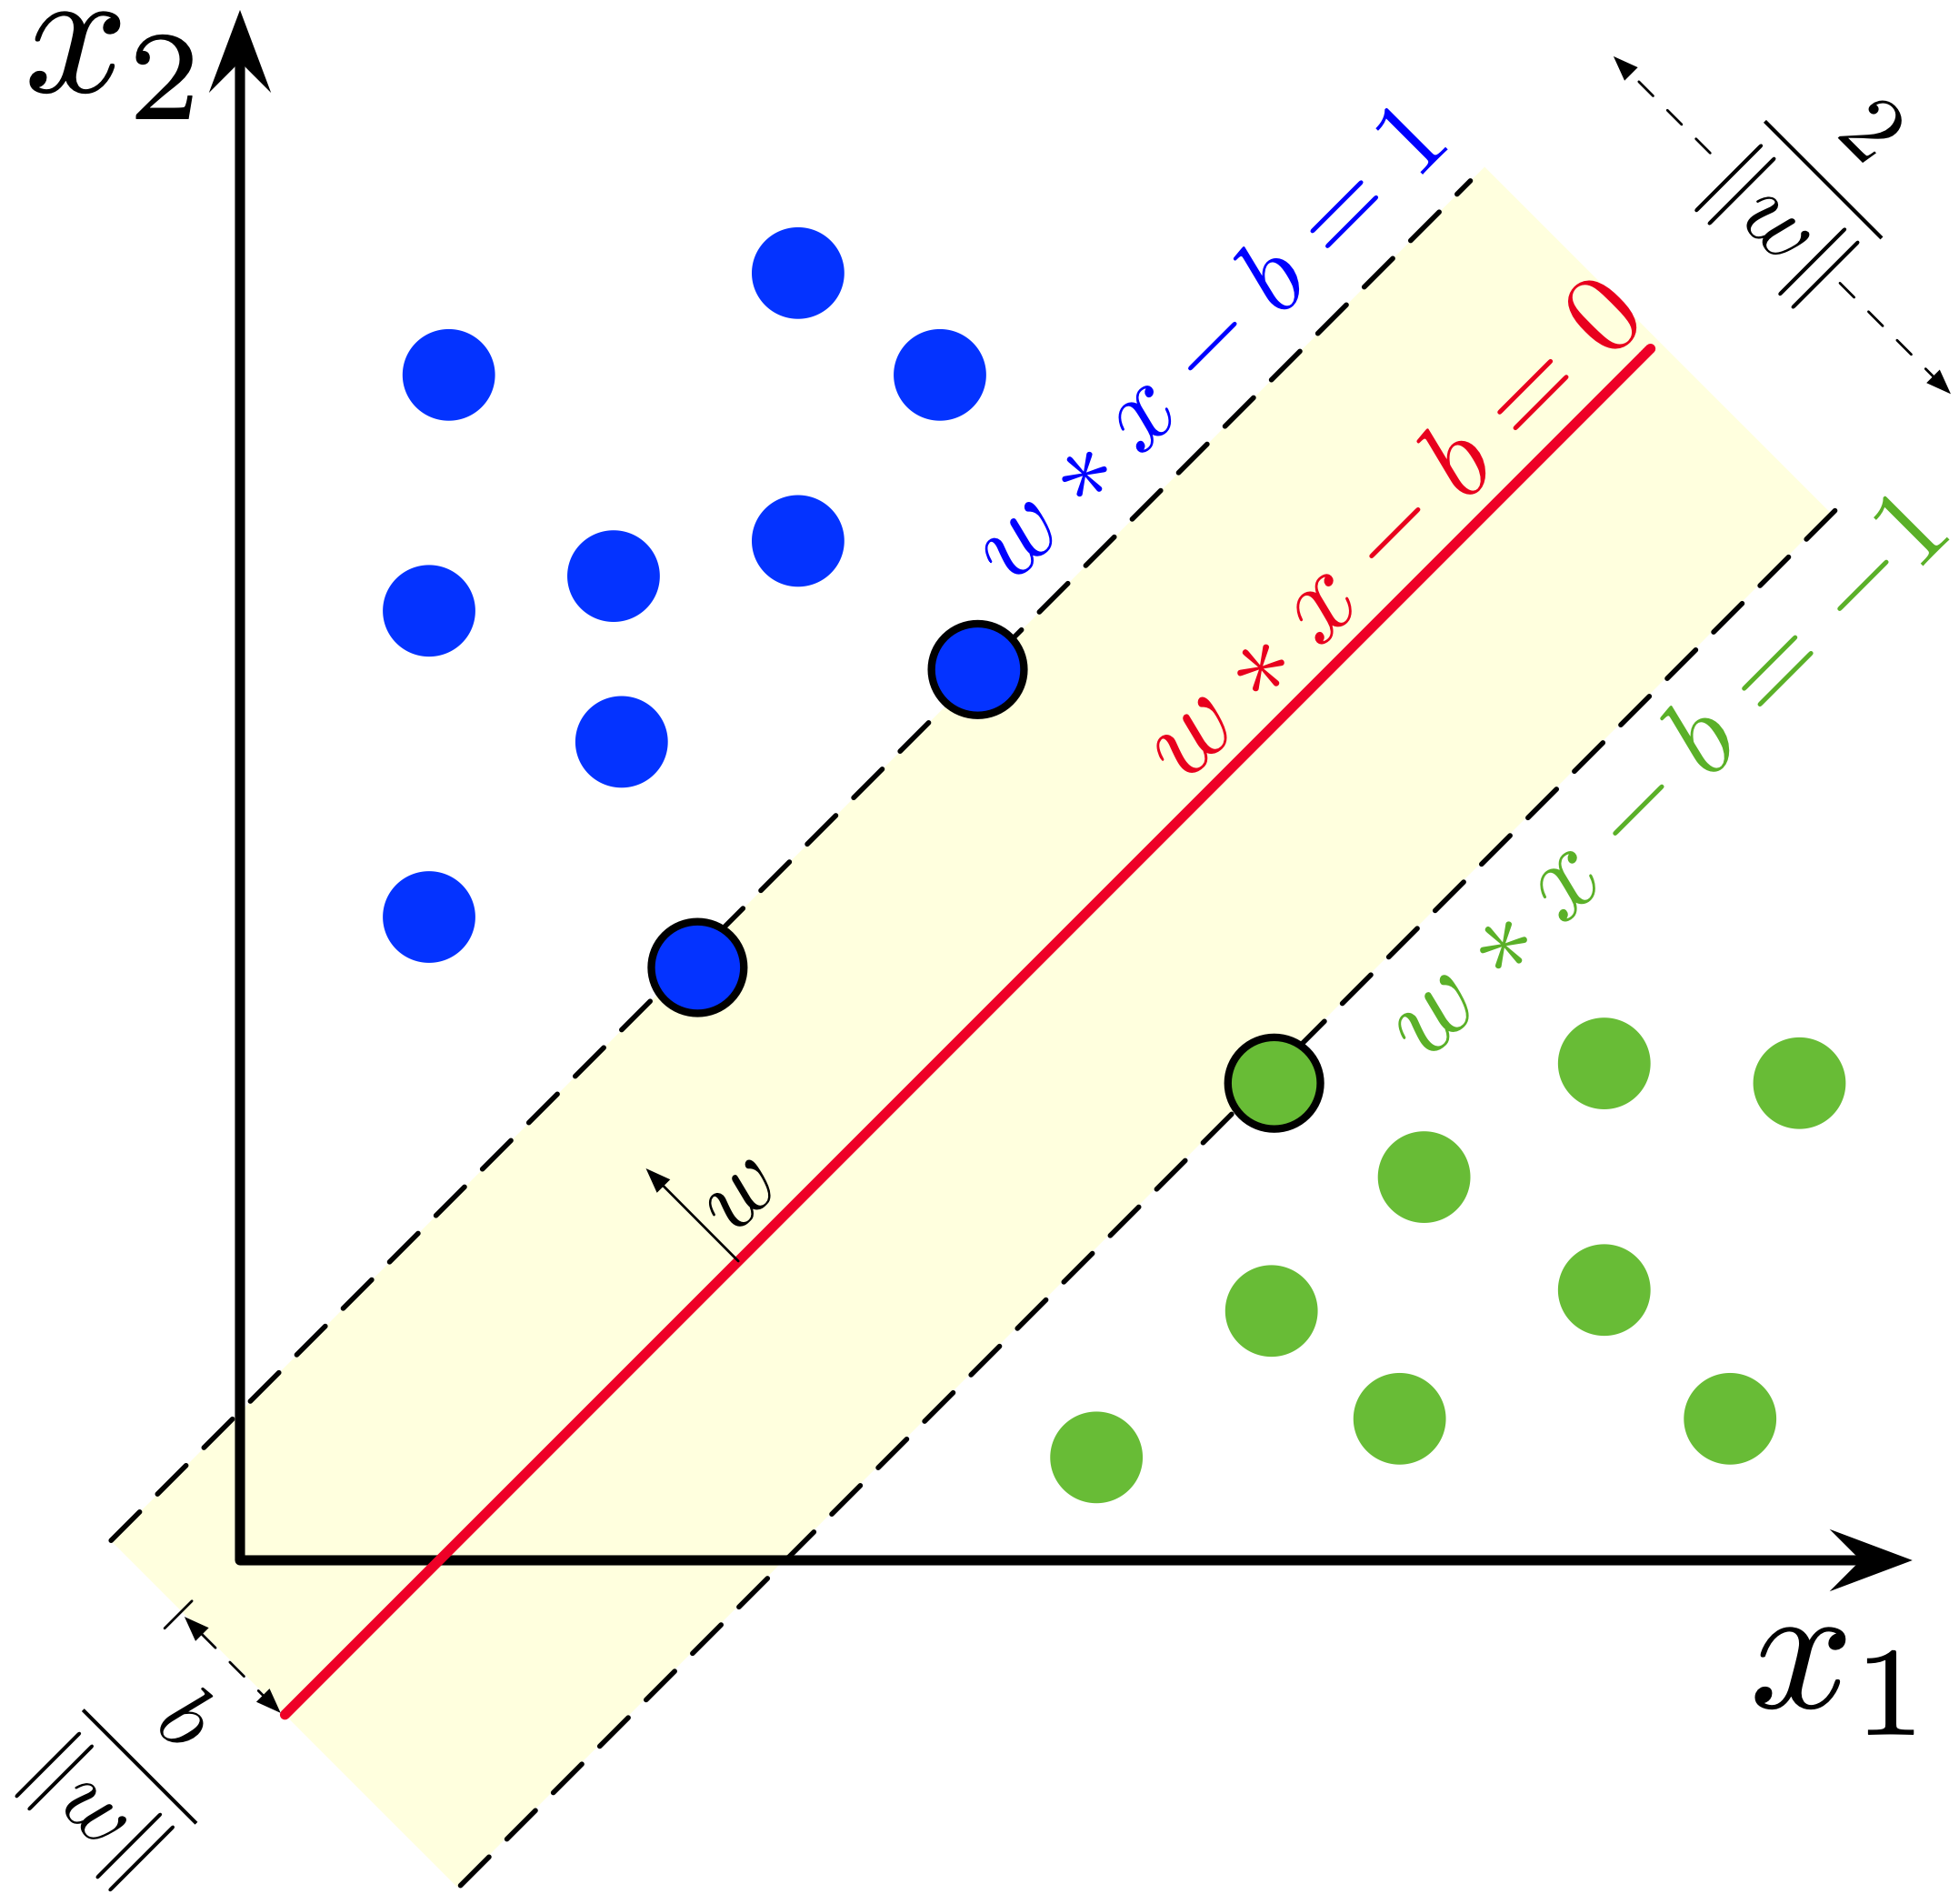
\includegraphics[width=.3\linewidth]{SVM_margin.png}
% % 	\caption{linearly separable SVM}
% % \end{figure}
% construct the classifier
% \begin{equation}
% 	\tilde{y}_{\textup{pred}}(\vb{s}) := \textup{sign} \qty(
% 		\sum_{i=1}^t y_i \alpha_i^* \kernel(\vbx_i,\vb{s}) + b
% 	)
% \end{equation}

% \subsubsection{Neural network}

\subsubsection{Quantum machine learning}\label{sec:quantum_machine_learning}
overview \cite{biamonteQuantumMachineLearning2017}
\begin{itemize}
	\item supervised learning: quantum SVM \cite{rebentrostQuantumSupportVector2014}, quantum neural network  \cite{congQuantumConvolutionalNeural2019}; 
	\item unsupervised learning: quantum PCA \cite{lloydQuantumPrincipalComponent2014} \cite{tangQuantumPrincipalComponent2021}.
	\item reinforcement learning:
	\item generative models:
\end{itemize}
% graph neural networks (GNNs) have emerged as an alternative to graph kernels.

\subsection{Group theory and symmetries}
permutation (symmetric) group $\mathbb{S}_n$;

\subsubsection{Representation theory}\label{sec:representation_theory}
group $\group$

\section{Symmetries in physics}
\subsection{Lagrangian formalism}\label{sec:lagrangian}
In optics, Fermat's principle states that the path taken by a ray between two given points is the path that can be traveled in the least (extremum) time. 
% Lagrange multiplier method
A similar argument, \emph{principle of least action}, was developed in classical mechanics:
% [\emph{Principle of least action}]
% postulate
% \begin{postulate}
% \end{postulate}
\begin{axiom}[Principle of least action]\label{thm:least_action}
    The actual path $q(t)$ taken by a classical system is the path that 
	yields an extremum of its action \(\action\).
	So, this principle is also called principle of stationary action.
	% or \emph{Hamilton's principle}.
	The action of the dynamics is the integral of Lagrangian over time
	\begin{equation}
		\action[q(t)]:=\int_{t_I}^{t_F}\dlagrangian(q(t),\dot{q}(t);t)\dd{t}
		\label{eq:action}
	\end{equation}
	where $\lagrangian(q,\dot{q})$ is the Lagrangian in terms of generalized coordinate $q$ and velocity $\dot{q}$ at certain time $t$. 
\end{axiom}
The notion $\action[\cdot]$ reminds that action is a functional that takes a function (path) $q(t)$ as input.
% see \cref{sec:path_integral} for more detail.
% (the simplest case is cartesian corrdinates, can be spherical etc)
% In classical mechanics, it is the actual path in the Euclidean space. 
By varying the action, one have the equation of motion 
% (Eq.\ref{eq:euler_lagrange}) 
called \emph{Euler-Lagrange equation}.
% \begin{equation}
%     \pdv{\lagrangian}{q_a}-\dv{t}\pdv{\lagrangian}{\dot{q}_a}=0
% \end{equation}
This Lagrangian formalism was extended by Dirac \cite{diracAnalogyClassicalQuantum1945} and Feynman \cite{feynmanQuantumMechanicsPath2010} to explain quantum mechanics. 
\begin{axiom}[Path integral]\label{thm:path_integral}
    The amplitude (probability) of a quantum system evolving from $\ket{q_I}$ to $\ket{q_F}$ in a time interval can be evaluated by (functional) integrating over all possible paths with fixed initial and final position 
    \begin{equation}
		\mel{q_F}{e^{-\ii t\hhat/\hbar}}{q_I} =
        \int_{q(t_I)= q_F}^{q(t_F)=q_I} \D q \; e^{\ii \action[q]/\hbar}
    \end{equation}
	where the action defined in classical mechanics as \cref{eq:action}.
\end{axiom}
The Larangian (path integral) formalism of quantum mechanics is proved to be equivalent to the well-known \schrodinger equation \cref{eq:evolution} \cite[Chp4]{feynmanQuantumMechanicsPath2010} 
% (complete specification)
% \begin{equation}
%     \ii\hbar \dv{t} \ket{\psi(t)} = \hhat(t) \ket{\psi(t)}
% 	% \ket{\psi}=\sum_{q} \alpha_{q} \ket{q}$, $\sum_{q} \abs{\alpha_{q}}^2=1.
%     \label{eq:evolution}
% \end{equation}
which is a differential equation determining the evolution of quantum state.
In the classical limit (Planck's constant $\hbar\to 0$), \nameref{thm:path_integral} reduces to \nameref{thm:least_action}
because only the paths around the stationary point of the action contribute 
(the other paths' contributions frequently oscillate and cancel out).
% We have included a summary of the path integral formalism for various kinds of systems in \cref{sec:path_integral}.
\subsubsection{Path integral and quantum computing}
\cite{xuLagrangianFormalismQuantum2021}

\subsection{Symmetries in physics with Lagrangians}
\subsubsection{Z}
Ising model, $\integer_2$
% \begin{theorem}[Noether theorem]
% \end{theorem}

\subsubsection{U(1)}
\cite{kogutIntroductionLatticeGauge1979}
local, gauge symmetry

\subsubsection{SU(2)}
non-abelian, particle physics

\subsubsection{SO(1,3)}
Lorentz invariance

% \subsubsection{quantum neural network}\label{sec:quantum_neural_network}
% \subsection{Unsupervised: PCA}

\section{Hardness assumptions}
\begin{definition}[\NP]\label{def:np}
	\NP, \NP-hard, \NP-complete
\end{definition}
\begin{definition}[\sharpP]\label{def:sharpp}
	\sharpP
\end{definition}
\begin{definition}[QMA]\label{def:qma}
	QMA
\end{definition}
\begin{definition}[\BPP]\label{def:bpp}
	\BPP
\end{definition}
\begin{definition}[\BQP]\label{def:bqp}
	\BQP
\end{definition}